\documentclass[a4paper,10pt,twocolumn,english]{article}

% ============================================================================
% Packages
% ============================================================================

\usepackage{babel}
\usepackage[utf8]{inputenc}
\usepackage[T1]{fontenc}
\usepackage{lmodern}
\usepackage{amsmath,amssymb,amsthm,mathtools}
\usepackage{graphicx}
\usepackage{booktabs}
\usepackage{array}
\usepackage{tabularx}
\usepackage{longtable}
\usepackage{listings}
\usepackage[table]{xcolor}
\usepackage{hyperref}
\usepackage{url}
\makeatletter
\g@addto@macro\UrlBreaks{\do\/\do\.\do\_\do\-\do\*}
\makeatother
\Urlmuskip=0mu\relax
\usepackage{enumitem}
\usepackage{microtype}
\usepackage{cleveref}
\usepackage[font=small,labelfont=bf]{caption}
\usepackage{float}
\usepackage{tikz}
\usepackage{eso-pic}
\AddToShipoutPictureBG{%
  \AtPageCenter{\makebox(0,0){\rotatebox{45}{\scalebox{8}{\textcolor[gray]{0.9}{DRAFT}}}}}%
}
\usetikzlibrary{positioning,calc,arrows.meta}

% TikZ figure styles
\tikzset{
  figfont/.style={font=\scriptsize\sffamily},
  figbox/.style={draw, rounded corners=2pt, align=center, inner sep=4pt},
  figboxgray/.style={figbox, fill=gray!10},
  figsubbox/.style={figbox, fill=white},
  figsubboxgray/.style={figbox, fill=gray!5},
  figarrow/.style={-{Stealth[length=2mm]}, thick},
  figarrowstrong/.style={figarrow, line width=0.6pt},
}

% Reduce space between section number and title, prevent hyphenation in headings
\makeatletter
\renewcommand{\@seccntformat}[1]{\csname the#1\endcsname\hspace{0.5em}}
\renewcommand{\section}{\@startsection{section}{1}{\z@}%
  {-3.5ex \@plus -1ex \@minus -.2ex}%
  {2.3ex}%
  {\raggedright\normalfont\large\bfseries}}
\renewcommand{\subsection}{\@startsection{subsection}{2}{\z@}%
  {-3.25ex \@plus -1ex \@minus -.2ex}%
  {1.5ex}%
  {\raggedright\normalfont\normalsize\bfseries}}
\renewcommand{\subsubsection}{\@startsection{subsubsection}{3}{\z@}%
  {-3.25ex \@plus -1ex \@minus -.2ex}%
  {1.5ex}%
  {\raggedright\normalfont\small\bfseries}}
\makeatother

% ============================================================================
% Typography improvements
% ============================================================================

\raggedbottom                           % Consistent local spacing
\widowpenalty=10000                     % Prevent widows (single lines at top)
\clubpenalty=10000                      % Prevent orphans (single lines at bottom)
\displaywidowpenalty=10000              % Prevent widows after display math
\predisplaypenalty=50                   % Discourage break before display math
\postdisplaypenalty=50                  % Discourage break after display math
\setlength{\emergencystretch}{2em}      % Reduce overfull lines in narrow columns
\setlength{\columnsep}{16pt}            % Slightly wider gutter for two-column reading
\setlength{\parskip}{0pt plus 1pt}      % Flexible paragraph spacing
\setlength{\floatsep}{12pt plus 3pt minus 2pt}
\setlength{\textfloatsep}{14pt plus 3pt minus 2pt}
\setlength{\intextsep}{12pt plus 3pt minus 2pt}
\setlength{\tabcolsep}{4pt}
\renewcommand{\arraystretch}{1.08}
\renewcommand{\topfraction}{0.85}       % Allow more floats at top
\renewcommand{\bottomfraction}{0.85}    % Allow more floats at bottom
\renewcommand{\textfraction}{0.10}      % Require less text on float pages
\renewcommand{\floatpagefraction}{0.7}  % Fuller float pages
\setcounter{topnumber}{2}
\setcounter{bottomnumber}{1}
\setcounter{totalnumber}{3}
\setlist[itemize]{leftmargin=*, itemsep=2pt, topsep=3pt}
\setlist[enumerate]{leftmargin=*, itemsep=2pt, topsep=3pt}
\setlist[description]{leftmargin=0pt, labelindent=0pt, itemsep=2pt, topsep=3pt}

% ============================================================================
% Numbering by section
% ============================================================================

\makeatletter
\@addtoreset{figure}{section}
\renewcommand{\thefigure}{\thesection.\arabic{figure}}
\@addtoreset{table}{section}
\renewcommand{\thetable}{\thesection.\arabic{table}}
\makeatother
\numberwithin{equation}{section}

% ============================================================================
% Theorem environments
% ============================================================================

\newtheoremstyle{paperplain}%
{6pt}{6pt}{\itshape\raggedright}{}{\bfseries}{}{0pt}%
{\thmname{#1}\thmnumber{ #2}\thmnote{. #3}.\hfill\break}
\newtheoremstyle{paperdef}%
{6pt}{6pt}{\normalfont\raggedright}{}{\bfseries}{}{0pt}%
{\thmname{#1}\thmnumber{ #2}\thmnote{. #3}.\hfill\break}
\newtheoremstyle{paperremark}%
{6pt}{6pt}{\normalfont\raggedright}{}{\itshape}{}{0pt}%
{\thmname{#1}\thmnumber{ #2}\thmnote{. #3}.\hfill\break}

\theoremstyle{paperdef}
\newtheorem{definition}{Definition}[section]

\theoremstyle{paperplain}
\newtheorem{theorem}[definition]{Theorem}
\newtheorem{lemma}[definition]{Lemma}
\newtheorem{proposition}[definition]{Proposition}
\newtheorem{corollary}[definition]{Corollary}

\theoremstyle{paperdef}
\newtheorem{example}[definition]{Example}
\newtheorem{assumption}{Assumption Block}[section]

\theoremstyle{paperremark}
\newtheorem{remark}[definition]{Remark}

\theoremstyle{paperdef}
\newtheorem{assumptions}[assumption]{Assumption Block}

% ============================================================================
% Custom commands
% ============================================================================

\newcolumntype{L}[1]{>{\raggedright\arraybackslash}p{#1}}
\newcommand{\thead}[1]{\textbf{\raisebox{0pt}[2.2ex][0.8ex]{#1}}}

\newcommand{\Hbyz}{\ensuremath{\mathsf{H}_{\mathrm{byz}}}}
\newcommand{\DeliveryModel}{\ensuremath{\mathsf{DeliveryModel}}}
\newcommand{\Obssafe}{\ensuremath{\mathsf{Obs}_{\mathrm{safe}}^{\mathrm{byz}}}}
\newcommand{\Eqsafe}{\ensuremath{\mathsf{Eq}_{\mathrm{safe}}^{\mathrm{byz}}}}
\newcommand{\Ebyz}{\ensuremath{\mathcal{E}_{\mathrm{byz}}}}
\newcommand{\ByzSafe}{\ensuremath{\mathsf{ByzSafe}}}
\newcommand{\ByzChar}{\ensuremath{\mathsf{ByzChar}}}
\newcommand{\Coherent}{\ensuremath{\mathsf{Coherent}}}
\newcommand{\Harmony}{\ensuremath{\mathsf{Harmony}}}
\newcommand{\Admissible}{\ensuremath{\mathsf{Admissible}}}
\newcommand{\EnvelopeRel}{\ensuremath{\mathsf{EnvelopeRel}}}
\newcommand{\EnvelopeExact}{\ensuremath{\mathsf{EnvelopeExact}}}
\newcommand{\EnvelopeOK}{\ensuremath{\mathsf{EnvelopeOK}}}
\newcommand{\ConfigEquiv}{\ensuremath{\mathsf{ConfigEquiv}}}
\newcommand{\ExchangeEq}{\ensuremath{\mathsf{ExchangeEq}}}
\newcommand{\Obs}{\ensuremath{\mathsf{Obs}}}
\newcommand{\ProjStep}[2]{\ensuremath{\mathsf{ProjStep}_{#2}(#1)}}
\newcommand{\LocStep}[2]{\ensuremath{\mathsf{LocStep}_{#2}(#1)}}
\newcommand{\ProjLink}[1]{\ensuremath{\mathsf{ProjLinkStep}(#1)}}
\newcommand{\LocLink}[1]{\ensuremath{\mathsf{LocLinkStep}(#1)}}
\newcommand{\ProjDelegate}[1]{\ensuremath{\mathsf{ProjDelegateStep}(#1)}}
\newcommand{\LocDelegate}[1]{\ensuremath{\mathsf{LocDelegateStep}(#1)}}
\newcommand{\JointActive}[1]{\ensuremath{\mathsf{JointRealizable}_{\mathsf{active}}(#1)}}
\newcommand{\EqsafeConformance}{\ensuremath{\mathsf{EqsafeConformance}}}
\newcommand{\VMAdheres}{\ensuremath{\mathsf{VMAdheres}}}
\newcommand{\HasProfileCapabilities}{\ensuremath{\mathsf{HasProfileCapabilities}}}
\newcommand{\wf}{\ensuremath{\mathsf{wf}}}
\newcommand{\envG}{\ensuremath{\mathsf{envG}}}
\newcommand{\envD}{\ensuremath{\mathsf{envD}}}
\newcommand{\pathref}[1]{\texttt{#1}}
\newcommand{\eqnote}[1]{\par\noindent\textit{#1.}\par\vspace{2pt}}
\newcommand{\ABHStack}{Theorems~\ref{thm:harmony}, \ref{thm:erasure}, \ref{thm:delegation}, \ref{thm:minimality}, \ref{thm:conservation}, \ref{thm:envelope}, \ref{thm:normalization}, and~\ref{thm:adequacy}}

\newenvironment{citelist}{%
  \begin{list}{}{%
    \setlength{\leftmargin}{1.25em}%
    \setlength{\itemindent}{-1.25em}%
    \setlength{\itemsep}{2pt}%
    \setlength{\parsep}{0pt}%
    \setlength{\topsep}{3pt}}%
}{\end{list}}

\lstset{
  basicstyle=\ttfamily\footnotesize,
  keywordstyle=\color{blue},
  commentstyle=\color{gray},
  stringstyle=\color{red},
  breaklines=true,
  frame=leftline,
  rulecolor=\color{black!10},
  framerule=3pt,
  framesep=1em,
  columns=fullflexible,
  aboveskip=8pt,
  belowskip=8pt,
  xleftmargin=1.5em,
  literate={->}{$\to$\ }2 {forall}{$\forall$}1 {:=}{$\coloneqq$}2
}

% ============================================================================
% Document
% ============================================================================

\title{Harmony from Coherence in Asynchronous MPST:\\A Minimal Erasure Invariant for Classical Dynamics}
\author{Sam Hart Berman}
\date{\empty}

\begin{document}
\maketitle

\begin{abstract}
	We establish a Reconfiguration Harmony theorem for asynchronous MPST. Under well-formed
	\texttt{link} and delegation reconfiguration, projection commutes with reconfigured evolution.
	This gives a proof architecture for dynamic participant sets where topology change is a first-class
	semantic step. The inherited operational coherence invariant kernel is characterized
	in both directions and shown to admit an erasure characterization on active edges and to be the
	weakest admissible invariant for delegation safety (relative minimality). Safe delegation and
	composed-system conservation follow, including quantitative lift of
	\emph{Computable Dynamics for Asynchronous MPST}'s Lyapunov framework with conservation for pure reconfiguration and descent or budget
	certificates for transition choreographies. The behavioral boundary is characterized by an exact
	determinism envelope with soundness, realizability, and maximality. Exchange-normalized determinism
	with spatial-subtyping monotonicity is established. Observational adequacy links abstract and
	protocol proofs to VM adherence modulo envelope. All results are mechanized in Lean~4.
\end{abstract}

% ============================================================================
\section{Introduction}
\label{sec:introduction}
% ============================================================================

\subsection{Background}

Delegation and topology change are a primary failure point in MPST developments (Honda et al., 2008,
and Tirore et al., 2025). Many systems exclude these operations, or admit them operationally without
a theorem that connects choreography-level and local-level evolution.

In classical MPST, coherence primarily names global-type coherence and projectability
conditions, with later refinements of projection criteria (Honda et al., 2008; Honda et al., 2016;
Castagna et al., 2012; Majumdar et al., 2021). Logical lines also formulate
coherence as n-ary duality or proof compatibility (Carbone et al., 2015; Carbone et al., 2016; Carbone
et al., 2017), and data-certification extensions remain in the same global-projection discipline
(Toninho and Yoshida, 2017). In this paper, as in \emph{Coherence for Asynchronous Buffered MPST}, $\Coherent$ denotes
the inherited operational invariant on local environments and buffered traces.

This manuscript is intended for companion review and publication with
\emph{Coherence for Asynchronous Buffered MPST} and
\emph{Computable Dynamics for Asynchronous MPST}. Cross-paper references in this
text use companion-series dependencies.

\subsection{Contribution}

This paper addresses the reconfiguration gap with a commutation theorem, in the broader process-semantic tradition of operational correspondence and mobility (Hoare, 1985; Plotkin, 1981; Milner et al., 1992; Milner, 1999).

The central statement is Harmony under reconfiguration:
\begin{equation}
	\mathsf{project}\,\circ\,\mathsf{step}_{\mathsf{reconfig}}
	=
	\mathsf{localStep}_{\mathsf{reconfig}}\,\circ\,\mathsf{project}.
\end{equation}
for well-formed \texttt{link} and delegation operations with enabled post-reconfiguration steps. The
theorem development proceeds from commutation to characterization and runtime adherence. It
establishes erasure characterization of Coherence, safe delegation consequences, and relative minimality
over admissible invariants. It then proves composed-system conservation, exact envelope
characterization, exchange-normalized determinism with spatial monotonicity, and observational adequacy
with VM adherence.
The theorem order in this manuscript is dependency-driven rather than alphabetical.

The determinism-envelope layer follows a standard refinement-bound idea. One defines an admissible
behavior relation that captures implementation freedom while preserving safety-visible observations.
What is new here is an exact characterization for asynchronous MPST reconfiguration with soundness,
realizability, and maximality proved in one theorem stack and connected directly to runtime admission
and adherence evidence (Abadi and Lamport, 1991; Alpern and Schneider, 1985).

Equivalently, the envelope is a coarse-grained observational equivalence. It is the maximal admissible
blur between executions that still preserves certified safety-visible meaning, in the spirit of
noninterference and hyperproperty viewpoints (Goguen and Meseguer, 1982; Clarkson and Schneider, 2010).

Sharding correspondence follows a standard simulation view for distributed execution. A split execution
should preserve the same safety-visible meaning as a reference execution under explicit compatibility
assumptions (Lamport, 1978; Chandy and Lamport, 1985; Lynch, 1996). What is new here is an explicit
envelope contract for local and cross-machine sharding profiles that makes the admissible difference
class theorem-checkable and capability-gated at the VM bridge.

The envelope layer also admits a rate-distortion style reading. The reference semantics is the source,
VM and sharded executions are channels, and admission profiles are distortion constraints on safety-visible
observations (Shannon, 1948, and Cover and Thomas, 2006). Maximality then states that no strictly larger
distortion class preserves the same certified safety guarantees.

\begin{figure}[H]
	\centering
	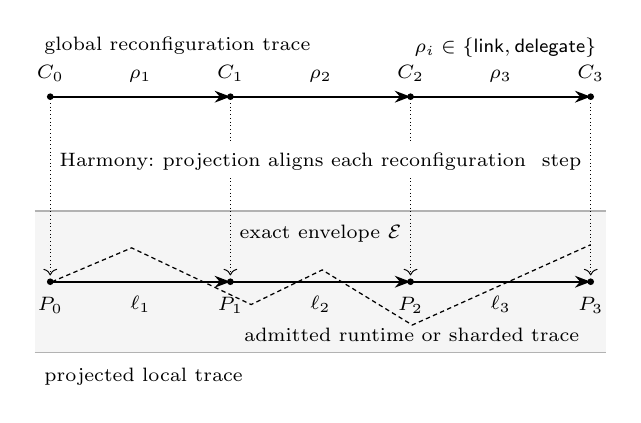
\begin{tikzpicture}[x=1.1mm,y=1mm,figfont]
		% Exact envelope corridor around local trace
		\fill[gray!8] (-33,-11.5) rectangle (33,6.5);
		\draw[gray!60, line width=0.5pt] (-33,6.5) -- (33,6.5);
		\draw[gray!60, line width=0.5pt] (-33,-11.5) -- (33,-11.5);
		\node[font=\scriptsize, align=center] at (0,3.6) {exact envelope $\mathcal{E}$};

		% Top: global reconfiguration trace
		\node[font=\scriptsize, anchor=west] at (-33,27.5) {global reconfiguration trace};
		\fill (-31.2,21.0) circle (1.2pt) node[above=2.0pt] {$C_0$};
		\fill (-10.4,21.0) circle (1.2pt) node[above=2.0pt] {$C_1$};
		\fill (10.4,21.0) circle (1.2pt) node[above=2.0pt] {$C_2$};
		\fill (31.2,21.0) circle (1.2pt) node[above=2.0pt] {$C_3$};
		\draw[figarrowstrong] (-31.2,21.0) -- node[above=1.5pt, font=\scriptsize] {$\rho_1$} (-10.4,21.0);
		\draw[figarrowstrong] (-10.4,21.0) -- node[above=1.5pt, font=\scriptsize] {$\rho_2$} (10.4,21.0);
		\draw[figarrowstrong] (10.4,21.0) -- node[above=1.5pt, font=\scriptsize] {$\rho_3$} (31.2,21.0);
		\node[font=\scriptsize, anchor=east] at (33,27.2)
		{$\rho_i\in\{\mathsf{link}, \mathsf{delegate}\}$};

		% Bottom: projected local trace
		\node[font=\scriptsize, anchor=west] at (-33,-14.6) {projected local trace};
		\fill (-31.2,-2.5) circle (1.2pt) node[below=2.0pt] {$P_0$};
		\fill (-10.4,-2.5) circle (1.2pt) node[below=2.0pt] {$P_1$};
		\fill (10.4,-2.5) circle (1.2pt) node[below=2.0pt] {$P_2$};
		\fill (31.2,-2.5) circle (1.2pt) node[below=2.0pt] {$P_3$};
		\draw[figarrowstrong] (-31.2,-2.5) -- node[below=1.5pt, font=\scriptsize] {$\ell_1$} (-10.4,-2.5);
		\draw[figarrowstrong] (-10.4,-2.5) -- node[below=1.5pt, font=\scriptsize] {$\ell_2$} (10.4,-2.5);
		\draw[figarrowstrong] (10.4,-2.5) -- node[below=1.5pt, font=\scriptsize] {$\ell_3$} (31.2,-2.5);

		% Projection alignments (Harmony correspondences)
		\draw[densely dotted, ->, line width=0.35pt] (-31.2,20.2) -- (-31.2,-1.7);
		\draw[densely dotted, ->, line width=0.35pt] (-10.4,20.2) -- (-10.4,-1.7);
		\draw[densely dotted, ->, line width=0.35pt] (10.4,20.2) -- (10.4,-1.7);
		\draw[densely dotted, ->, line width=0.35pt] (31.2,20.2) -- (31.2,-1.7);
		\node[font=\scriptsize, align=center] at (0,12.8)
		{Harmony:\colorbox{white}{projection aligns each reconfiguration} step};

		% In-band admissible runtime trace (piecewise-linear, crossing local transitions)
		\draw[dash pattern=on 1.6pt off 1.2pt, line width=0.45pt]
		(-31,-2.5) -- (-21.8,1.8) -- (-8,-5.4) -- (0.2,-1.0) --
		(10.6,-8) -- (31.2,2.2);
		\node[font=\scriptsize, align=right, anchor=east] at (31,-9.2)
		{admitted runtime or sharded trace};
	\end{tikzpicture}
	\caption{Dual-track trace view. Top track is the global reconfiguration trace
		$C_0 \to C_1 \to C_2 \to C_3$ labeled by $\rho_i$. Middle track is the
		projected local trace with corresponding labels $\ell_i$. Bottom band is the
		admitted runtime trace corridor inside envelope $\mathcal{E}$. The figure
		intentionally scopes to $\rho\in\{\mathsf{link},\mathsf{delegate}\}$; transition
		choreography is introduced later.}
	\label{fig:p3-layered-stack}
\end{figure}

\subsection{Scope}

This paper closes the series architecture. \emph{Coherence for Asynchronous Buffered MPST} supplies
the invariant kernel. \emph{Computable Dynamics for Asynchronous MPST} supplies bounds and decision
procedures. This paper supplies reconfiguration commutation and envelope-level runtime adherence.

Scope is confined to asynchronous buffered semantics with explicit reconfiguration conditions,
crash-stop fault assumptions where fault claims are stated, and declared envelope-admission profiles.

\begin{table}[H]
	\centering
	\scriptsize
	\begin{tabularx}{\columnwidth}{@{}L{0.27\columnwidth}L{0.68\columnwidth}@{}}
		\toprule
		\thead{Result}              & \thead{Imported Dependencies and Use}                                                                                                                                                          \\
		\midrule
		Harmony                     & Imports the Paper 1 Coherence preservation and replacement stack, and Paper 2 computable-step premises, then proves projection commutation under link and delegation updates.                  \\
		Minimality and Conservation & Imports the Paper 1 active-edge Coherence kernel, and Paper 2 transition-side quantitative premises, then fixes invariant minimality and conservation under declared reconfiguration premises. \\
		Envelope family             & Imports the Paper 1 quotient-facing Coherence boundary, and Paper 2 profile extraction interfaces, then lifts the safety core to envelope exactness, normalization, and VM adherence claims.   \\
		Byzantine family            & Imports the Paper 2 Byzantine safety interface and converse packaging, then extends this interface to envelope-level maximality and adherence transport.                                       \\
		\bottomrule
	\end{tabularx}
	\caption{Series dependency map for Paper 3.}
	\label{tab:p3-series-dependencies}
\end{table}

In Table~\ref{tab:p3-series-dependencies}, Harmony corresponds to Theorem~\ref{thm:harmony}. Minimality and Conservation correspond to Theorems~\ref{thm:minimality} and~\ref{thm:conservation}. Envelope family corresponds to Theorems~\ref{thm:envelope}, \ref{thm:normalization}, and~\ref{thm:adequacy}. Byzantine family corresponds to Theorem~\ref{thm:byzantine}, Corollary~\ref{cor:byzantine-converse}, and Proposition~\ref{prop:byzantine-vm}.

\begin{table}[H]
	\centering
	\scriptsize
	\begin{tabularx}{\columnwidth}{@{}L{0.16\columnwidth}L{0.79\columnwidth}@{}}
		\toprule
		\thead{Paper} & \thead{Byzantine Layer Added}                                                                                 \\
		\midrule
		Paper 1       & Interface obligations and bridge-ready Byzantine requirement classes.                                         \\
		Paper 2       & Profile-level exact safety characterization plus converse witness packaging for dropped assumptions.          \\
		Paper 3       & Reconfiguration-compatible exactness and capability-gated VM adherence/admission under the envelope boundary. \\
		\bottomrule
	\end{tabularx}
	\caption{Cross-paper Byzantine progression.}
	\label{tab:p3-byz-progression}
\end{table}

Our contributions are as follows:
\begin{enumerate}
	\item A reconfiguration commutation theorem that covers both static composition and dynamic delegation.
	\item An exact characterization of Coherence by active-edge erasure realizability and a relative-minimality theorem over admissible invariants.
	\item A determinism-envelope theory with soundness, realizability, maximality, and exchange and spatial normalization consequences.
	\item An abstract-to-VM adequacy bridge that ties profile claims to theorem-pack capability evidence.
	\item A Byzantine envelope extension with exact characterization, converse counterexample families, and capability-gated VM adherence.
\end{enumerate}

Main text proofs are proof sketches; full machine-checked derivations are provided by the Lean anchors indexed in Appendix~\ref{app:index}.
Proof-sketch template used throughout the series: state proof mode
(compositional/induction/coinduction/witness construction), give one concrete
intermediate transformation, then conclude with the claim interface.

\begin{table}[H]
	\centering
	\footnotesize
	\begin{tabularx}{\columnwidth}{@{}L{0.34\columnwidth}L{0.61\columnwidth}@{}}
		\toprule
		\thead{Symbol}               & \thead{Meaning}                                                  \\
		\midrule
		\Hbyz                        & Byzantine characterization bundle                                \\
		\Obssafe                     & Byzantine safety-visible observation                             \\
		\Eqsafe                      & Byzantine safety-visible equality                                \\
		\Ebyz                        & Byzantine determinism-envelope                                   \\
		\Coherent                    & global active-edge coherence predicate                           \\
		\Harmony                     & reconfiguration commutation invariant                            \\
		$\Admissible(I)$             & candidate invariant admissibility                                \\
		$W$                          & weighted state function                                          \\
		$\mathcal{E}$                & determinism-envelope trace set (admitted behaviors)              \\
		\EnvelopeRel                 & envelope relation between VM and reference states                \\
		\EnvelopeExact               & exactness of envelope characterization                           \\
		\EnvelopeOK                  & envelope-admission predicate                                     \\
		$\mathsf{Cap}_{\mathcal{E}}$ & capability set admitted by the envelope profile                  \\
		\ConfigEquiv{}               & erasure-stability equivalence                                    \\
		\Obs                         & observation map on executions/states                             \\
		$C,\ C_i$                    & configuration state(s) used in reconfiguration traces            \\
		$P_i$                        & projected-local trace nodes in Figure~\ref{fig:p3-layered-stack} \\
		$p,\Pi$                      & runtime profile pair used in capability/adherence statements     \\
		\ByzChar                     & Byzantine characterization formula                               \\
		\ByzSafe                     & Byzantine safety predicate                                       \\
		$\mathsf{HasCaps}(p,\Pi)$    & capability-evidence predicate for profile $(p,\Pi)$              \\
		\VMAdheres                   & VM adherence predicate under admitted profile                    \\
		$N_s$                        & explored state count in finite checker objects                   \\
		$N_e$                        & explored transition-edge count in finite checker objects         \\
		$L_{\max}$                   & maximum active-edge buffered trace length                        \\
		$W_{\max}$                   & maximum size of checked witness/certificate object               \\
		$\ell$                       & projected local-step label for reconfiguration steps             \\
		$\rho$                       & reconfiguration step label (link/delegate/transition)            \\
		\bottomrule
	\end{tabularx}
	\caption{Notation used in this paper.}
	\label{tab:p3-notation}
\end{table}

% ============================================================================
\section{Setup, Definitions, and Side Conditions}
\label{sec:setup}
% ============================================================================

\subsection{Base Recap}

Assume the base model from \emph{Coherence for Asynchronous Buffered MPST} and \emph{Computable Dynamics for Asynchronous MPST}: asynchronous buffered steps, active-edge Coherence, fair scheduling assumptions stated per theorem, \DeliveryModel parametricity, and crash-stop setting for fault claims.

\begin{table}[H]
	\centering
	\small
	\begin{tabularx}{\columnwidth}{@{}L{0.55\columnwidth}L{0.4\columnwidth}@{}}
		\toprule
		\thead{Assumption}                       & \thead{Status}         \\
		\midrule
		async buffered semantics                 & required               \\
		active-edge Coherence                    & required               \\
		reconfig.\ conditions $\mathsf{WF}_\rho$ & required               \\
		fair scheduling profile                  & req.\ where stated     \\
		crash-stop fault model                   & req.\ for fault claims \\
		\bottomrule
	\end{tabularx}
	\caption{Model assumptions for exact claims in this paper.}
	\label{tab:p3-model-assumptions}
\end{table}

\begin{assumptions}[Core Model]
	\label{assump:p3-core}
	Core claims in this paper assume asynchronous buffered semantics, active-edge Coherence,
	reconfiguration side conditions through $\mathsf{WF}_\rho$, and the stated fairness profile.
	Crash-stop premises apply where fault-side claims are stated.
\end{assumptions}

Assumption-block inheritance policy. Assumption blocks do not inherit implicitly. If a theorem does not name a block, it uses Assumption Block~\ref{assump:p3-core} only.

\begin{definition}[Well-Typed Reconfiguration Configuration and Step]
	Write $\Gamma \vdash C\ \wf$ for configuration typing and
	$\Gamma \vdash C \xrightarrow{\rho} C'$ for typed reconfiguration steps under
	the declared operator profile.
\end{definition}

Role split. Well-typedness enforces operator and update side conditions for
reconfiguration steps. Coherence enforces active-edge compatibility invariants
transported through those steps.

\subsection{Reconfiguration Operators}

The paper distinguishes static composition (\texttt{link}) in deployment-level composition from dynamic delegation (endpoint/capability transfer during execution). Representative mechanized anchors are in the deployment-composition layer, the delegation-preservation layer, and the higher-order graph-delta layer. Appendix~\ref{app:index} provides the file-level mapping.

\subsection{Dynamic Participant Sets}

Participant sets are not fixed: participants may join through delegation, leave through crash-stop or transfer-and-exit, or change topology through composition.

The objective is to preserve Coherence/Harmony across these mutations.

\subsection{Core Definitions}

Write $\envG(C)$ and $\envD(C)$ for the global and delayed-trace environments extracted from
configuration $C$, and $\Obs$ for the safety-visible observation map.

\begin{definition}[Lifted Coherence]
	\begin{equation}
		\Coherent(C) := \Coherent(\envG(C), \envD(C)).
	\end{equation}
\end{definition}

\begin{definition}[Projection Operator]
	\label{def:p3-project}
	$\mathsf{project}$ is the canonical projection from reconfiguration configurations to local-step configurations used by the Harmony square. The mechanized definition is \texttt{project} in \texttt{Runtime/\allowbreak Adequacy/\allowbreak EnvelopeCore/\allowbreak ReconfigurationBridge.lean}.
\end{definition}

\begin{definition}[Harmony]
	For reconfiguration operator $\rho$,
	\begin{equation}
		\begin{aligned}[t]
			\Harmony(C,\rho)
			 & :\iff \ProjStep{C}{\rho} \\
			 & =
			\LocStep{C}{\rho}.
		\end{aligned}
	\end{equation}
\end{definition}

Here $\ProjStep{C}{\rho}$ abbreviates
$\mathsf{project}(\mathsf{step}_{\mathsf{reconfig}}(C,\rho))$,
and $\LocStep{C}{\rho}$ abbreviates
$\mathsf{localStep}_{\mathsf{reconfig}}(\mathsf{project}(C),\rho)$.

Figure~\ref{fig:p3-commuting-square} gives the explicit commuting-square instance for Harmony.
\begin{figure}[H]
	\centering
	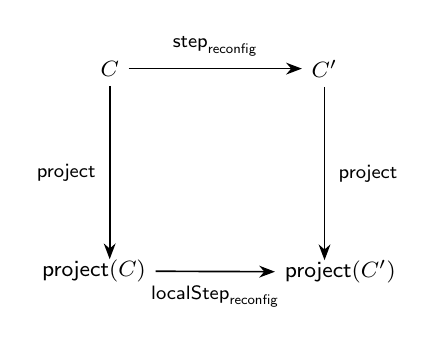
\begin{tikzpicture}[figfont, node distance=22mm]
		% Corner nodes
		\node[font=\footnotesize\sffamily] (TL) {$C$};
		\node[right=of TL, font=\footnotesize\sffamily] (TR) {$C'$};
		\coordinate[below=of TL] (BL);
		\coordinate[below=of TR] (BR);
		\node[font=\footnotesize\sffamily, xshift=-2mm, yshift=-1.5mm] (BLlbl) at (BL) {$\mathsf{project}(C)$};
		\node[font=\footnotesize\sffamily, xshift=2mm, yshift=-1.5mm] (BRlbl) at (BR) {$\mathsf{project}(C')$};

		% Horizontal arrows
		\draw[figarrowstrong] (TL) -- node[above=1.0pt, font=\scriptsize] {$\mathsf{step}_{\mathsf{reconfig}}$} (TR);
		\draw[figarrowstrong] (BLlbl) -- node[below=1.5pt, font=\scriptsize] {$\mathsf{localStep}_{\mathsf{reconfig}}$} (BRlbl);

		% Vertical arrows
		\draw[figarrowstrong] (TL) -- node[left=1.5pt, font=\scriptsize] {$\mathsf{project}$} (BL);
		\draw[figarrowstrong] (TR) -- node[right=1.5pt, font=\scriptsize] {$\mathsf{project}$} (BR);
	\end{tikzpicture}

	\vspace{4pt}
	{\footnotesize $\rho\in\{\mathsf{link},\mathsf{delegate}\}$}
	\caption{Commuting-square formulation of Harmony. Horizontal arrows are global
		reconfiguration and projected-local reconfiguration. Vertical arrows are
		projection. Commutation states that projecting after one reconfiguration step
		equals stepping in the projected local model.}
	\label{fig:p3-commuting-square}
\end{figure}

\begin{definition}[Joint Realizability on Active Edges]
	$\mathsf{JointRealizable}_{\mathsf{active}}(\mathsf{project}(C))$ holds when projected
	local views admit witnesses for all active edges.
\end{definition}

\begin{definition}[Reconfiguration Well-Formedness]
	Write $\mathsf{WF}_\rho(C)$ for the side-condition predicate used by reconfiguration theorems:
	\texttt{LinkWF(C,$\rho$)} for static linking, \texttt{DelegationWF(C,$\rho$)} for delegation,
	and \texttt{TransitionWF(C,$\rho$)} for transition choreographies.
\end{definition}

\begin{definition}[Transition Well-Formedness Obligations]
	\label{def:p3-transition-wf}
	$\mathsf{TransitionWF}(C,\rho_{\mathsf{tr}})$ holds when all of the following
	are discharged.
	\begin{enumerate}
		\item Structural typing and domain stability: source/target interfaces are
		      well-typed, endpoint and edge domains are preserved on untouched
		      components, and the declared transition footprint is well-formed.
		\item Transition enabledness: the mode-transition operator is enabled at $C$
		      under the declared operational side conditions.
		\item Profile-premise package: $\mathsf{TrPrem}(C)$ is available, including
		      scheduler/budget-side evidence used by transition descent arguments.
		\item Trigger and guard discharge: declared transition trigger predicates
		      and typed guard predicates are both satisfied.
	\end{enumerate}
\end{definition}

\begin{definition}[TransitionWF Judgment Schema]
	\label{def:p3-transition-wf-schema}
	For transition choreography $\rho_{\mathsf{tr}}$, define witness package
	\[
		\omega_{\mathsf{tr}} := (\omega_{\mathsf{ty}},\omega_{\mathsf{en}},\omega_{\mathsf{pr}},\omega_{\mathsf{gd}})
	\]
	and judgment
	\begin{equation}
		\label{eq:p3-transitionwf-schema}
		\begin{aligned}[t]
			\mathsf{TransitionWF}(C,\rho_{\mathsf{tr}})
			 & :\iff \exists \omega_{\mathsf{tr}}.\,
			\mathsf{TyDomStable}(C,\rho_{\mathsf{tr}};\omega_{\mathsf{ty}})
			\\
			 & \land \mathsf{TrEnabled}(C,\rho_{\mathsf{tr}};\omega_{\mathsf{en}})
			\\
			 & \land \mathsf{TrPrem}(C;\omega_{\mathsf{pr}})
			\\
			 & \land \mathsf{GuardedTr}(C,\rho_{\mathsf{tr}};\omega_{\mathsf{gd}}).
		\end{aligned}
	\end{equation}
	Items 1--4 of Definition~\ref{def:p3-transition-wf} correspond to
	$\mathsf{TyDomStable}$, $\mathsf{TrEnabled}$, $\mathsf{TrPrem}$, and
	$\mathsf{GuardedTr}$ respectively.
\end{definition}

Obligation split. Items 1--3 in Definition~\ref{def:p3-transition-wf} are
structural proof obligations. Item 4 records application-level transition
triggers together with typed admissibility guards.

\begin{definition}[Delegation Safety Predicates]
	$\mathsf{SafeDelegation}(C,\rho_{\mathsf{del}})$ is the global delegation-safety judgment, and
	$\mathsf{SafeDelegationFootprint}(C,\rho_{\mathsf{del}})$ is its footprint-local form over edges touched by $\rho_{\mathsf{del}}$.
\end{definition}

\begin{definition}[$\Admissible(I)$]
	$\Admissible(I)$ holds iff all of the following obligations are satisfied:
	\begin{enumerate}
		\item Locality: $I$ is checkable from edge-local obligations on active edges.
		\item Erasure stability: $I$ is preserved under \ConfigEquiv classes.
		\item Frame stability: untouched edges/endpoints preserve $I$ under context extension.
		\item Delegation-footprint adequacy: for each delegation step $\rho_{\mathsf{del}}$, $I$ entails the footprint-local update obligations used by Equation~\ref{eq:p3-delegation-footprint} together with the declared $\mathsf{WF}_{\rho_{\mathsf{del}}}$ side conditions.
	\end{enumerate}
\end{definition}

Admissibility is defined by these obligations only. It does not assume \Coherent.

\begin{definition}[Envelope Predicates]
	Write
	\[
		\begin{aligned}[t]
			\EnvelopeRel(S_{\mathrm{vm}}, S_{\mathrm{ref}})
			 & := \mathsf{ObsEq}(S_{\mathrm{vm}}, S_{\mathrm{ref}})            \\
			 & \land \mathsf{CertStepAlign}(S_{\mathrm{vm}}, S_{\mathrm{ref}}) \\
			 & \land \mathsf{ProfileAlign}(S_{\mathrm{vm}}, S_{\mathrm{ref}}).
		\end{aligned}
	\]
	$\mathsf{ObsEq}$ means safety-visible observations agree.
	$\mathsf{CertStepAlign}$ means every admitted VM step has the declared certified-step witness in the reference layer.
	$\mathsf{ProfileAlign}$ means both states satisfy the same profile-side admission obligations.
	$\EnvelopeExact(C)$ is exactness of the declared envelope (soundness and
	realizability and maximality) at configuration $C$. $\EnvelopeOK(C)$ means $C$ satisfies
	the envelope-admission obligations used in Theorems~\ref{thm:envelope}--\ref{thm:normalization}.
\end{definition}

Concrete example. Let $S_{\mathrm{ref}}$ be a reference execution prefix for the running example up to $\rho_2$. Let $S_{\mathrm{vm}}$ be a VM execution prefix with the same admitted external events, plus internal monitor bookkeeping steps. If the bookkeeping steps are silent at $\Obs$, certified-step witnesses map each admitted VM step to the same reference prefix, and both prefixes satisfy the same profile obligations, then $\EnvelopeRel(S_{\mathrm{vm}}, S_{\mathrm{ref}})$ holds.

Construction recipe. To instantiate $\EnvelopeRel$ for a new protocol, first fix the safety-visible observation map $\Obs$. Second, define the certified-step witness relation used by the admission checker. Third, define profile-side admission obligations and use their conjunction with observation equality and certified-step alignment.

\begin{definition}[Capability/Adherence Predicates]
	$\HasProfileCapabilities(p,\Pi)$ means profile $(p,\Pi)$ is backed by required theorem-pack
	capability evidence. $\VMAdheres(p,\Pi)$ means executions admitted under $(p,\Pi)$ satisfy
	the corresponding adherence obligations.
\end{definition}

\begin{definition}[Configuration Equivalence (\ConfigEquiv)]
	\label{def:p3-config-equiv}
	\ConfigEquiv\ is the least reflexive/symmetric/transitive closure of the
	base generator relation below, and is closed under context extension on
	untouched components (congruence at the frame boundary):
	\begin{enumerate}
		\item silent internal administrative steps that preserve safety-visible
		      observations,
		\item endpoint-preserving renamings on configuration identifiers,
		\item frame-preserving bookkeeping rewrites on untouched components.
	\end{enumerate}
\end{definition}

Cross-paper notation note. Paper 1 writes this same quotient relation as
$\sim$. Canonical alias for coherent/admitted states is:
\[
	X \sim Y \iff X\ \ConfigEquiv\ Y.
\]
Paper 1 uses $\sim$ for readability in early quotient equations, while this
paper uses \ConfigEquiv\ to align theorem and mechanization names.

\begin{table}[H]
	\centering
	\footnotesize
	\begin{tabularx}{\columnwidth}{@{}L{0.36\columnwidth}L{0.59\columnwidth}@{}}
		\toprule
		\thead{Generator (paper)}  & \thead{Lean anchor/module mapping}                                                                            \\
		\midrule
		silent admin steps         & \nolinkurl{config_equiv_iff_effect_bisim_silent} (\texttt{Runtime/Proofs/EffectBisim/ConfigEquivBridge.lean}) \\
		endpoint renamings         & \texttt{Protocol/Coherence/ConfigEquivRenaming/*.lean}                                                        \\
		frame bookkeeping rewrites & \texttt{Protocol/Coherence/ConfigEquiv.lean}                                                                  \\
		\bottomrule
	\end{tabularx}
	\caption{Mapping from paper-level \ConfigEquiv\ generators to mechanized anchors/modules.}
	\label{tab:p3-config-equiv-map}
\end{table}

Observation-preservation note. By construction, every generator in
Definition~\ref{def:p3-config-equiv} preserves the safety-visible interface
$\Obs$, so \ConfigEquiv\ is an observational quotient.

\begin{lemma}[Generator Sanity for \ConfigEquiv]
	\label{lem:p3-config-equiv-generator-sanity}
	If $C \Rightarrow_{\mathsf{gen}} C'$ by one generator from
	Definition~\ref{def:p3-config-equiv}, then
	$\Obs(C)=\Obs(C')$.
\end{lemma}

\begin{proof}[Proof sketch]
	Proof mode: case analysis on generator family. Silent administrative steps are
	\Obs-silent by definition, renamings preserve endpoint-level observations, and
	frame bookkeeping rewrites leave observed components untouched. Hence each
	generator preserves \Obs.
\end{proof}

\begin{definition}[Normalization Relations]
	$\ExchangeEq$ is the least equivalence relation generated by adjacent swaps of independent reconfiguration steps. A swap is admissible when two enabled steps $\rho_a,\rho_b$ from the same pre-state $C$ satisfy all of the following.
	\begin{enumerate}
		\item Footprints are disjoint:
		      $\mathsf{Footprint}(\rho_a)\cap\mathsf{Footprint}(\rho_b)=\varnothing$.
		\item Both orders are enabled from $C$ under declared $\mathsf{WF}_\rho$ side conditions.
		\item Diamond commutation holds at the update boundary:
		      \[
			      C \xrightarrow{\rho_a} C_a \xrightarrow{\rho_b} C_{ab},
			      \qquad
			      C \xrightarrow{\rho_b} C_b \xrightarrow{\rho_a} C_{ba},
		      \]
		      and $C_{ab}\ \ConfigEquiv\ C_{ba}$.
	\end{enumerate}
	Then $\ExchangeEq(C_1,C_2)$ holds when $C_1$ and $C_2$ are connected by a finite sequence of such admissible swaps plus \ConfigEquiv closure.
	$C \sqsubseteq_{\mathsf{sp}} C'$ is the spatial-subtyping preorder used in Theorem~\ref{thm:normalization}.
\end{definition}

Relation inclusion and role split. Because \ExchangeEq\ is closed under
\ConfigEquiv, we have
\[
	C_1\ \ConfigEquiv\ C_2 \implies C_1\ \ExchangeEq\ C_2.
\]
\ConfigEquiv\ is the observational quotient used by erasure and adequacy
statements. \ExchangeEq\ extends this with independent-step commutations used by
exchange normalization.

Concrete exchange example. Suppose $C$ has two enabled reconfiguration steps with disjoint footprints, one \texttt{link} step and one delegation step on a different session edge. If both orders are well-formed and produce \ConfigEquiv post-states, then the two resulting configurations are exchange-equivalent.

\begin{definition}[Non-Interference Across Composition]
	$\mathsf{NonInterf}(C_1,C_2)$ holds iff all of the following hold.
	\begin{enumerate}
		\item Footprint disjointness: boundary write footprints of enabled steps from $C_1$ and $C_2$ are disjoint.
		\item Boundary commutation: if one enabled step from each component can fire, both execution orders are defined and preserve the same safety-visible observation.
		\item Witness factorization: certified-step witnesses for composed traces factor into component witnesses without cross-boundary dependencies.
	\end{enumerate}
\end{definition}

Checkability note. Under the same finite-reachability regime used in Paper 2,
Clause 1 is decidable by finite footprint-set intersection. Clause 2 is
decidable by bounded two-step exploration of enabled boundary transitions. Clause
3 is decidable when certified-step witnesses are represented by finite proof
objects with total checkers. In that regime, checker/verifier complexity is
$\mathrm{poly}(N_s+N_e)$ with witness-validation overhead
$\mathrm{poly}(W_{\max})$. This is a validation bound, distinct from runtime
transition-step cost in admitted executions.

Scope boundary. Outside finite-reachability or finite-witness encodings, this
paper does not claim a total non-interference decider.

Equation~\ref{eq:p3-delegation-footprint} states the delegation-footprint update discipline.
\begin{equation}
	\label{eq:p3-delegation-footprint}
	\begin{aligned}[t]
		C'                            & := \mathsf{step}_{\mathsf{reconfig}}(C,\rho_{\mathsf{del}}), \\
		F                             & := \mathsf{Footprint}(\rho_{\mathsf{del}}),                  \\
		D                             & := \envD(C),\ D' := \envD(C'),                               \\
		G                             & := \envG(C),\ G' := \envG(C'),                               \\
		\forall e\in F,\quad D'(e)    & =\mathsf{rewrite}(D(e),\rho_{\mathsf{del}}),                 \\
		\forall e\notin F,\quad D'(e) & =D(e),                                                       \\
		G'                            & = G\ \text{on untouched endpoints.}
	\end{aligned}
\end{equation}

% ============================================================================
\section{Worked Example}
\label{sec:example}
% ============================================================================

We extend the baseline protocol through a sequence of reconfigurations, including federation, delegation, and mode transition, demonstrating how harmony, safety, and budget conservation compose at each step. The example carries the full structural theorem stack (\ABHStack) and shows that coherence-preserving reasoning from the first paper lifts through these dynamic changes.

\noindent\begingroup\raggedright
\textbf{Running example.} Baseline choreography:
\par\endgroup

\noindent\begin{minipage}{\columnwidth}
	\begin{lstlisting}
C -> P : Request(n)
P -> C : Grant(k)
C -> M : Report(k)
M -> P : Confirm
P -> C : Token(t)
\end{lstlisting}
\end{minipage}

Extended system adds: \texttt{link} federation (\texttt{P1}, \texttt{P2}),
delegation $C \to C'$, and optimistic-to-coordinated transition choreography.

Fix configurations and reconfiguration operators:
\begin{equation}
	C_0 \xrightarrow{\rho_{\mathsf{link}}} C_1 \xrightarrow{\rho_{\mathsf{del}}}
	C_2 \xrightarrow{\rho_{\mathsf{tr}}} C_3.
\end{equation}
Assume well-formedness judgments $\Gamma \vdash C_i\ \wf$ for $i=0,1,2,3$. Here $C_0$ is the coherent single-pool state before federation, $C_1$ is the linked/federated state, $C_2$ is the post-delegation state where token capability is held by $C'$, and $C_3$ is the coordinated-mode state after transition choreography.

The running obligations are used through these derived rule instances.
Write $\mathsf{TrPrem}(C)$ for the transition-profile premise package at $C$, and
$\mathsf{BDesc}(C,C')$ for a budget-certified descent witness from $C$ to $C'$.

	{\small
		\begin{equation}
			\begin{aligned}
				\mathsf{SD}(C,\rho)        & := \mathsf{SafeDelegation}(C,\rho);                      \\
				\mathsf{SDF}(C,\rho)       & := \mathsf{SafeDelegationFootprint}(C,\rho);             \\
				\mathsf{EnvRel}^{\star}(C) & := \EnvelopeRel(S_{\mathsf{vm}}(C),S_{\mathsf{ref}}(C)); \\
				\mathsf{ObsEq}^{\star}(C)  & := \Obs(S_{\mathsf{vm}}(C))=\Obs(S_{\mathsf{ref}}(C)).
			\end{aligned}
		\end{equation}
	}
\eqnote{Example derivation: link harmony}
{\small
	\begin{equation}
		\dfrac{
		\Gamma \vdash C_0\ \wf;\ \mathsf{WF}_{\rho_{\mathsf{link}}}(C_0)
		}{
		\ProjStep{C_0}{\rho_{\mathsf{link}}}
		=
		\LocStep{C_0}{\rho_{\mathsf{link}}}
		}
	\end{equation}
}
\eqnote{Example derivation: delegation safety}
{\small
	\begin{equation}
		\dfrac{
			\Coherent(C_1);\ \mathsf{DelegationWF}(C_1,\rho_{\mathsf{del}})
		}{
			\mathsf{SD}(C_1,\rho_{\mathsf{del}});\ \mathsf{SDF}(C_1,\rho_{\mathsf{del}})
		}
	\end{equation}
}
\eqnote{Example derivation: conservation}
{\small
	\begin{equation}
		\dfrac{
		\mathsf{WF}_{\rho_{\mathsf{link}}}(C_0);\ \Coherent(C_0)
		}{
		W(C_1)=W(C_0)
		}
	\end{equation}
}
\eqnote{Example derivation: transition}
{\small
	\begin{equation}
		\dfrac{
		\mathsf{WF}_{\rho_{\mathsf{tr}}}(C_2);\ \Coherent(C_2);\ \mathsf{TrPrem}(C_2)
		}{
		C_2 \to^\ast C_3;\ \mathsf{BDesc}(C_2,C_3)
		}
	\end{equation}
}
\eqnote{Example derivation: adequacy and adherence}
{\small
	\begin{equation}
		\dfrac{
			\mathsf{EnvRel}^{\star}(C_3);\ \HasProfileCapabilities(p,\Pi)
		}{
			\mathsf{ObsEq}^{\star}(C_3);\ \VMAdheres(p,\Pi)
		}
	\end{equation}
}

Table~\ref{tab:p3-typed-guards} gives the typed guard clauses used to discharge $\mathsf{WF}_{\rho_{\mathsf{tr}}}$
for the optimistic-to-coordinated step.

\begin{table}[H]
	\centering
	\scriptsize
	\begin{tabularx}{\columnwidth}{@{}L{0.29\columnwidth}L{0.31\columnwidth}L{0.30\columnwidth}@{}}
		\toprule
		\thead{Guard}                                 & \thead{Source}     & \thead{Consequence} \\
		\midrule
		\texttt{conflict\_detected}                   & app-level trigger  & transition enabled  \\
		\texttt{reachable}\allowbreak\texttt{(Coord)} & crash decider      & path preserved      \\
		$W \leq \text{budget}$                        & quant.\ bound      & budget-feasible     \\
		$|F| \leq f$                                  & fault-budget decl. & bounded tolerance   \\
		\bottomrule
	\end{tabularx}
	\caption{Typed guard clauses for transition well-formedness.}
	\label{tab:p3-typed-guards}
\end{table}

Guard-to-predicate link. The rows of Table~\ref{tab:p3-typed-guards} discharge
Item 4 of Definition~\ref{def:p3-transition-wf}: \texttt{conflict\_detected} is
the application trigger, while \texttt{reachable(Coord)}, budget feasibility,
and fault-budget bounds are typed/profile guards.
At equation level, the same rows build the guard witness used in
Equation~\ref{eq:p3-transitionwf-schema}:
\begin{equation}
	\label{eq:p3-guard-discharge}
	\frac{
		\begin{array}{c}
			\mathsf{conflict\_detected}(C_2;\omega_{\mathsf{trg}})
			\quad
			\mathsf{reachable}_{\mathsf{Coord}}(C_2;\omega_{\mathsf{reach}})
			\\
			W(C_2)\le \mathsf{budget}(\omega_{\mathsf{budget}})
			\quad
			|F(C_2)|\le f(\omega_{\mathsf{fault}})
		\end{array}
	}{
		\mathsf{GuardedTr}(C_2,\rho_{\mathsf{tr}};\omega_{\mathsf{gd}})
	}
\end{equation}
Combining \eqref{eq:p3-guard-discharge} with
$\omega_{\mathsf{ty}},\omega_{\mathsf{en}},\omega_{\mathsf{pr}}$ yields
$\mathsf{TransitionWF}(C_2,\rho_{\mathsf{tr}})$ by
Equation~\ref{eq:p3-transitionwf-schema}.

Concrete reading: $C_0$ pre-federation, $C_1$ linked, $C_2$ post-delegation handoff, $C_3$
coordinated mode with preserved envelope obligations.

% ============================================================================
\section{Theorem B: Reconfiguration Harmony (Static + Dynamic)}
\label{sec:theorem-b}
% ============================================================================

Running-example thread. Section~\ref{sec:example} instantiates this theorem on
the sequence $C_0 \xrightarrow{\rho_{\mathsf{link}}} C_1
	\xrightarrow{\rho_{\mathsf{del}}} C_2$.

Reading-order note. Theorem~\ref{thm:harmony} is presented before
Theorem~\ref{thm:erasure} because later statements depend first on
reconfiguration commutation and only then on erasure characterization.
Appendix~\ref{app:regimes} Figure~\ref{fig:p3-dependency-graph}
gives the full dependency graph for this ordering.

\begin{assumptions}[Reconfiguration]
	\label{assump:p3-reconfiguration}
	The reconfiguration theorems assume typed global and local states, reconfiguration
	witnesses satisfying $\mathsf{WF}_\rho$, enabled post-reconfiguration steps, and
	compatibility side conditions for unaffected edges.
\end{assumptions}

\begin{theorem}[Reconfiguration Harmony]
	\label{thm:harmony}
	For all configurations $C$ and reconfiguration operators $\rho \in \{\mathsf{link},
		\mathsf{delegate}\}$, if Assumption Block~\ref{assump:p3-reconfiguration} holds for $(C,\rho)$, then
	\begin{equation}
		\ProjStep{C}{\rho}
		=
		\LocStep{C}{\rho}.
	\end{equation}
	Equivalently, the reconfiguration square commutes at the projection boundary.
\end{theorem}

Premise roles. In Theorem~\ref{thm:harmony}, typedness discharges
$\mathsf{WF}_{\rho}$ obligations for \texttt{link}/\texttt{delegate}, while
Coherence is the preserved safety invariant transported through commutation.

Running-example instantiation. For the example in
Section~\ref{sec:example}, the link and delegation steps are exactly the two
operators in this theorem.

\begin{lemma}[Delegation Projection Preservation Shape]
	\label{lem:p3-deleg-proj-shape}
	Under Assumption Block~\ref{assump:p3-reconfiguration}, let $\rho_{\mathsf{del}}$ be a well-formed delegation step from $C$ with footprint $F$ and post-state $C'=\mathsf{step}_{\mathsf{reconfig}}(C,\rho_{\mathsf{del}})$. If the update discipline of Equation~\ref{eq:p3-delegation-footprint} holds, then
	\begin{equation}
		\mathsf{project}(C')
		=
		\mathsf{localStep}_{\mathsf{reconfig}}(\mathsf{project}(C),\rho_{\mathsf{del}}).
	\end{equation}
\end{lemma}

The lemma packages the delegate case used in Theorem~\ref{thm:harmony}. On footprint edges $e\in F$, projection follows delegation update witnesses. On non-footprint edges $e\notin F$, projection follows frame preservation. These two clauses are exactly the commutation link from update discipline to projected-step equality.

The proof has two components: static Harmony via \texttt{link}, where composition-level commutation and coherence preservation are established in deployment theorems such as \nolinkurl{link_harmony_through_link} and \nolinkurl{link_preserves_coherent}; and dynamic Harmony via delegation, where delegation preservation and footprint lemmas establish commutation for topology-changing transfers. At the effect-observation boundary, the coinductive bridge supplies the composition-facing
congruence and quotient lift used by this section: \nolinkurl{effect_bisim_congr_link} and
\nolinkurl{config_equiv_iff_effect_bisim_silent}.

Side-condition necessity is explicit. Dropped-condition counterexample interfaces are part
of the reconfiguration bridge layer.

\begin{proof}
	Fix $C$ and $\rho\in\{\mathsf{link},\mathsf{delegate}\}$ satisfying
	Assumption Block~\ref{assump:p3-reconfiguration}. We prove
	\[
		\ProjStep{C}{\rho}=\LocStep{C}{\rho}
	\]
	by case analysis on $\rho$.

	\textbf{Case $\rho=\mathsf{link}$.}
	From $\mathsf{WF}_\rho$ we obtain a well-formed composition object and enabled post-link step.
	Apply \nolinkurl{link_preserves_coherent} to preserve coherence across the link update, then apply
	\nolinkurl{link_harmony_through_link} to obtain commutation of projection with the link step:
	\[
		\begin{aligned}[t]
			\mathsf{project}(\mathsf{step}_{\mathsf{reconfig}}(C,\mathsf{link}))
			 & = \\
			\mathsf{localStep}_{\mathsf{reconfig}}(\mathsf{project}(C),\mathsf{link}).
		\end{aligned}
	\]
	This is exactly $\ProjStep{C}{\mathsf{link}}=\LocStep{C}{\mathsf{link}}$.

	\textbf{Case $\rho=\mathsf{delegate}$.}
	Let $F:=\mathsf{Footprint}(\rho_{\mathsf{del}})$ and write
	$C':=\mathsf{step}_{\mathsf{reconfig}}(C,\rho_{\mathsf{del}})$.
	Delegation well-formedness gives the side conditions required by the delegation-preservation layer.
	Apply Lemma~\ref{lem:p3-deleg-proj-shape} to the same $C,\rho_{\mathsf{del}},F$,
	i.e. $\ProjStep{C}{\mathsf{delegate}}=\LocStep{C}{\mathsf{delegate}}$.
	In the running example, this is the $C_1 \to C_2$ delegation handoff.

	\textbf{Boundary transport.}
	The above equalities are preserved at the observational/quotient interface by
	\nolinkurl{effect_bisim_congr_link} and
	\nolinkurl{config_equiv_iff_effect_bisim_silent}, so the same commutation statement holds at the
	composition-facing boundary used by later theorems.

	Both cases are proved, therefore $\ProjStep{C}{\rho}=\LocStep{C}{\rho}$ for all
	$\rho\in\{\mathsf{link},\mathsf{delegate}\}$ under the stated assumptions.
\end{proof}

Equation~\ref{eq:p3-commutation-instances} separates static-link and dynamic-delegation commutation instances.
\eqnote{Commutation instances: link and delegate}
\begin{equation}
	\label{eq:p3-commutation-instances}
	\begin{aligned}[t]
		\ProjLink{C}     & = \LocLink{C};     \\
		\ProjDelegate{C} & = \LocDelegate{C}.
	\end{aligned}
\end{equation}

% ============================================================================
\section{Theorem A: Projection-Erasure Characterization of Coherence}
\label{sec:theorem-a}
% ============================================================================

Running-example thread. Section~\ref{sec:example} provides the concrete
projected traces used to read this equivalence operationally.

Erasure terminology. This paper uses three related terms. Projection erasure is
the map $\mathsf{project}$. Class erasure is quotienting by \ConfigEquiv.
Finite-state erasure transportability is the boundary property in
Corollary~\ref{cor:transportability}.

\begin{theorem}[Projection-Erasure Characterization of Coherence]
	\label{thm:erasure}
	Under Assumption Block~\ref{assump:p3-core}, for all configurations $C$,
	\begin{equation}
		\begin{aligned}[t]
			\Coherent(C)
			\\
			\iff\ \JointActive{\mathsf{project}(C)}.
		\end{aligned}
	\end{equation}
	That is, Coherence holds exactly when projected local views admit a compatible active-edge witness assignment.
\end{theorem}

Running-example instantiation. For $C_0,\dots,C_3$ in
Section~\ref{sec:example}, the theorem identifies Coherence with active-edge
realizability of their projected local views.

This theorem gives the formal content of the quotient-first claim: erasure is not a heuristic post-processing step but the semantic object preserved by the theorem stack.

\begin{proof}[Proof sketch]
	The two directions are proved separately.

	\begin{enumerate}
		\item $\Coherent \to \mathsf{JointRealizable}_{\mathsf{active}}$:
		      \begin{itemize}
			      \item from edge-local compatibility ($\mathsf{EdgeCoherent}$) build per-edge witnesses for projected local obligations,
			      \item combine witnesses over active edges to obtain joint realizability.
		      \end{itemize}
		\item $\mathsf{JointRealizable}_{\mathsf{active}} \to \Coherent$:
		      \begin{itemize}
			      \item invert witness assignment into edge-local consume compatibility,
			      \item reassemble edge obligations into global $\Coherent$.
		      \end{itemize}
		\item Class-erasure stability:
		      \begin{itemize}
			      \item use \nolinkurl{coherent_erasure_stable} to show equivalence is preserved across configuration erasure classes.
		      \end{itemize}
	\end{enumerate}

	Therefore Coherence is exactly characterized by active-edge realizability of projected views.
\end{proof}

% ============================================================================
\section{Theorem C: Safe Delegation with Footprint Corollary}
\label{sec:theorem-c}
% ============================================================================

Running-example thread. Section~\ref{sec:example} uses this theorem at the
delegation step $\rho_{\mathsf{del}}$ from $C_1$ to $C_2$.

\begin{theorem}[Safe Delegation Sufficiency]
	\label{thm:delegation}
	Under Assumption Block~\ref{assump:p3-reconfiguration}, for all configurations $C$ and delegation operations $\rho_{\mathsf{del}}$,
	\begin{equation}
		\begin{aligned}[t]
			\Coherent(C) \land \mathsf{DelegationWF}(C,\rho_{\mathsf{del}})
			\\
			\implies\ \mathsf{SafeDelegation}(C,\rho_{\mathsf{del}}).
		\end{aligned}
	\end{equation}
\end{theorem}

Running-example instantiation. The delegation operation in
Section~\ref{sec:example} is a direct instance of this theorem's premise shape.

\begin{corollary}[Footprint Exactness Packaging]
	\label{cor:footprint}
	Under Assumption Block~\ref{assump:p3-reconfiguration}, for all $C,\rho_{\mathsf{del}}$ satisfying the stated step and well-formedness side conditions,
	\begin{equation}
		\begin{aligned}[t]
			\mathsf{SafeDelegation}(C,\rho_{\mathsf{del}})
			\\
			\iff\ \mathsf{SafeDelegationFootprint}(C,\rho_{\mathsf{del}}).
		\end{aligned}
	\end{equation}
	The converse direction is accompanied by strictness witnesses for dropped side conditions.
\end{corollary}

\begin{proof}[Proof sketch]
	Sufficiency follows by composing:
	\begin{enumerate}
		\item Coherence on active edges,
		\item delegation well-formedness side conditions ($\mathsf{WF}_{\rho_{\mathsf{del}}}$),
		\item delegation-preservation lemmas that update only the delegation footprint.
	\end{enumerate}
	Together these imply safe delegation without introducing additional global invariants.
\end{proof}

\begin{proof}[Proof sketch]
	For the forward direction, apply \nolinkurl{safe_delegation_to_footprint} to project $\mathsf{SafeDelegation}$ obligations to the declared delegation footprint. For the reverse direction, apply \nolinkurl{footprint_to_safe_delegation} to reconstruct global safety from footprint obligations. Strictness witnesses from \nolinkurl{safe_delegation_local_necessity} show necessity of the side conditions. The full equivalence is packaged as \nolinkurl{safe_delegation_iff_footprint}.
\end{proof}

% ============================================================================
\section{Theorem D: Relative Minimality}
\label{sec:theorem-d}
% ============================================================================

Running-example thread. Section~\ref{sec:example} gives the concrete
admissibility obligations that this minimality theorem abstracts.

\begin{theorem}[Relative Minimality]
	\label{thm:minimality}
	Under Assumption Block~\ref{assump:p3-reconfiguration}, for all invariants $I$,
	\begin{equation}
		\begin{aligned}[t]
			\Admissible(I)
			 & \implies \forall C,\ I(C) \\
			 & \implies \Coherent(C).
		\end{aligned}
	\end{equation}
	Hence Coherence is the weakest admissible invariant that guarantees delegation safety under the stated model side conditions.
\end{theorem}

Running-example instantiation. For the running reconfiguration sequence, any
candidate invariant used to certify delegation safety must imply the same
Coherence core.

This theorem prevents ``stronger-than-needed'' invariant inflation and pins down the architectural core.
It is a characterization-style minimality theorem relative to the admissibility class above.

\begin{proof}[Proof sketch]
	Assume any invariant $I$ satisfying $\Admissible(I)$.

	\begin{enumerate}
		\item Use admissibility clauses (locality, erasure stability, frame stability, delegation adequacy) to transport $I$ along the same edge-local transformations used by Coherence.
		\item Apply delegation-safety adequacy to derive local safety obligations on all active edges.
		\item Convert these obligations into Coherence via erasure-characterization lemmas.
	\end{enumerate}

	The full minimality statement is packaged as \nolinkurl{relative_minimality}. Hence every admissible safety-guaranteeing invariant implies Coherence, making Coherence relatively minimal.
\end{proof}

Equation~\ref{eq:p3-admissible-order} summarizes the admissible-invariant order behind Theorem~\ref{thm:minimality}.
The display below separates the invariant implication layer from its delegation
safety consequence so the proof flow remains explicit.
\begin{equation}
	\label{eq:p3-admissible-order}
	\begin{array}{c}
		\Admissible(I)
		\\
		\Downarrow
		\\
		\forall C,\ I(C)\Rightarrow \Coherent(C)
		\\
		\Downarrow
		\\
		\text{delegation safety consequences}.
	\end{array}
\end{equation}

% ============================================================================
\section{Theorem E: Composed-System Conservation}
\label{sec:theorem-e}
% ============================================================================

Running-example thread. Section~\ref{sec:example} instantiates the pure-link and
delegation conservation path before transition choreography descent.

\begin{theorem}[Composed-System Conservation]
	\label{thm:conservation}
	Under Assumption Block~\ref{assump:p3-reconfiguration}, for all configurations $C$ and reconfiguration operators $\rho$, if $\mathsf{WF}_\rho(C)$ and $\Coherent(C)$ hold, then
	\begin{equation}
		\Coherent(\mathsf{step}_{\mathsf{reconfig}}(C,\rho)).
	\end{equation}
	For all configurations $C$ and pure reconfiguration operators $\rho$,
	\begin{equation}
		\begin{aligned}[t]
			\mathsf{WF}_\rho(C) \land \Coherent(C)
			\\
			\implies\ W(\mathsf{step}_{\mathsf{reconfig}}(C,\rho)) = W(C).
		\end{aligned}
	\end{equation}
	For transition choreographies $\rho_{\mathrm{tr}}$ with stated budget and scheduler premises (fairness-required), descent and budget certificates are preserved with conservative profile-dependent bounds.
\end{theorem}

Fairness-required clause. The pure-reconfiguration conservation statements are
fairness-independent. The transition-side bounded-dissipation clause uses the
declared scheduler/fairness premises imported with the quantitative profile.

Running-example instantiation. In Section~\ref{sec:example}, $C_0 \to C_1 \to
	C_2$ is the conservative branch and $C_2 \to C_3$ is the budgeted transition
branch.

The theorem separates conservation and dissipation roles. Pure reconfiguration preserves the weighted quantity exactly. Transition choreographies consume certified progress budget and are therefore dissipative with explicit bounds. This split keeps structural rewiring distinct from progress-consuming work.

Under composition and delegation:
\begin{enumerate}
	\item Coherence and Harmony are preserved.
	\item Quantitative lift from \emph{Computable Dynamics for Asynchronous MPST} holds:
	      \begin{itemize}
		      \item pure reconfiguration conserves the weighted measure,
		      \item transition choreographies are governed by descent and budget certificates.
	      \end{itemize}
\end{enumerate}

This theorem combines composition, delegation, and quantitative invariants in one package.

\begin{proof}[Proof sketch]
	Split reconfiguration into conservative and budgeted classes.

	\begin{enumerate}
		\item Pure reconfiguration (\texttt{link}/delegation):
		      \begin{itemize}
			      \item preserve Coherence/Harmony by Theorem~\ref{thm:harmony}-side machinery,
			      \item show weighted measure $W$ is invariant under balanced delegation/rewiring (\nolinkurl{lyapunov_conserved_under_balanced_delegation}).
		      \end{itemize}
		\item Transition choreographies:
		      \begin{itemize}
			      \item apply inherited quantitative descent/budget certificates from the dynamics layer,
			      \item conclude bounded dissipation under declared scheduler premises.
		      \end{itemize}
		\item Compose both cases via \nolinkurl{flagship_composed_system_conservation} to obtain theorem statement and conservative profile-dependent quantitative side.
	\end{enumerate}
\end{proof}

\begin{corollary}[Compositional Exactness Under Non-Interference]
	\label{cor:compositional}
	For all compositions $C_1 \otimes C_2$, if Assumption Block~\ref{assump:p3-envelope} holds for both components and $\mathsf{NonInterf}(C_1,C_2)$ holds, then envelope exactness is preserved by composition:
	\begin{equation}
		\begin{aligned}
			\EnvelopeExact(C_1) \land \EnvelopeExact(C_2)
			 & \implies \\
			\EnvelopeExact(C_1 \otimes C_2).
		\end{aligned}
	\end{equation}
	Strictness witnesses are provided for dropped non-interference premises.
\end{corollary}

\begin{proof}[Proof sketch]
	$\mathsf{NonInterf}(C_1,C_2)$ gives a check criterion through footprint disjointness and boundary commutation, and a semantic criterion through witness factorization. These clauses factor composed traces into component traces with no cross-boundary interference steps. Apply envelope exactness to each component and recompose to obtain exactness of the composition. For strictness, use the dropped-assumption witness family to exhibit an interfering trace that violates factorization and therefore exactness.
\end{proof}

Interference example. If both components perform delegation rewrites that target the same boundary edge in one macro-step window, footprint disjointness fails. The two execution orders can then induce different certified boundary traces, so composed exactness can fail.

Equation~\ref{eq:p3-quantitative-split} summarizes the quantitative split.
The next display separates pure conservation from transition-side descent to
match the two proof branches in Theorem~\ref{thm:conservation}.
Write $S_\rho(C):=\mathsf{step}_{\mathsf{reconfig}}(C,\rho)$.
\begin{equation}
	\label{eq:p3-quantitative-split}
	\begin{aligned}[t]
		\mathsf{pure}  & \Rightarrow W(S_\rho(C)) = W(C),      \\
		\mathsf{trans} & \Rightarrow \mathsf{descent\_budget}.
	\end{aligned}
\end{equation}
Here $\mathsf{pure}$ abbreviates pure reconfiguration, and $\mathsf{trans}$ abbreviates transition choreography with inherited descent/budget certification under the stated profile assumptions.

% ============================================================================
\section{Theorem F: Exact Characterization of Determinism Envelope}
\label{sec:theorem-f}
% ============================================================================

Running-example thread. Section~\ref{sec:example} supplies the admitted
execution prefixes used to read the envelope clauses.

\begin{assumptions}[Envelope]
	\label{assump:p3-envelope}
	Envelope theorems assume the declared admissibility profile with trace well-formedness, certified-step obligations, and the realizability witness schema used by the admission checker.
\end{assumptions}

\begin{theorem}[Exact Determinism Envelope]
	\label{thm:envelope}
	Under Assumption Block~\ref{assump:p3-envelope}, there exists an envelope relation \EnvelopeRel and an induced admitted trace set $\mathcal{E}$ such that:
	\begin{enumerate}
		\item Soundness: $\forall t,\ \mathsf{Certified}(t) \implies t \in \mathcal{E}$.
		\item Realizability: $\forall t \in \mathcal{E},\ \exists e,\ \mathsf{Trace}(e) = t$.
		\item Maximality: $\forall \mathcal{E}'$, if $\mathcal{E}' \supsetneq \mathcal{E}$, then $\exists t \in \mathcal{E}' \setminus \mathcal{E}$ that violates admissibility constraints.
	\end{enumerate}
\end{theorem}

Running-example instantiation. The admitted traces around $C_3$ in
Section~\ref{sec:example} are the concrete profiles for soundness and
realizability checks.

The envelope claim is exact under the stated model and assumption bundle:
\begin{enumerate}
	\item soundness: certified executions lie within the envelope.
	\item realizability and completeness: admitted envelope behaviors are witnessed.
	\item maximality: strict supersets are rejected by witness counterexamples.
\end{enumerate}

Conceptually, this is dual to Theorem~\ref{thm:minimality}:
\begin{itemize}
	\item D: weakest admissible invariant core,
	\item F: maximal admissible behavior envelope.
\end{itemize}

\begin{proof}[Proof sketch]
	Exactness is obtained by packaging three envelope properties.

	\begin{enumerate}
		\item Soundness:
		      \begin{itemize}
			      \item derive $\mathsf{Certified} \to \mathsf{Envelope}$ from local/sharded envelope soundness definitions and profile extraction.
		      \end{itemize}
		\item Realizability/completeness:
		      \begin{itemize}
			      \item use realizability witness schemas to construct executions for admitted envelope behaviors.
		      \end{itemize}
		\item Maximality:
		      \begin{itemize}
			      \item show any strict envelope extension violates admissibility via explicit witness obligations.
		      \end{itemize}
	\end{enumerate}

	Core formal structures come from envelope foundations (\texttt{LocalExactEnvelopeCharacterization}, \texttt{ShardedExactEnvelopeCharacterization}) and profile-level extraction theorems (\nolinkurl{consensus_envelope_exact_of_profile},\allowbreak\ \nolinkurl{failure_envelope_maximality_of_profile}).
	Method split. Soundness/maximality steps are compositional consequence
	packaging over certified-step obligations, while realizability is a witness
	construction argument that builds executions from admitted traces.
\end{proof}

\begin{corollary}[Finite-State Erasure-Transportability Boundary]
	\label{cor:transportability}
	Under Assumption Block~\ref{assump:p3-envelope},
	\begin{equation}
		\begin{aligned}[t]
			\forall t,\ \mathsf{FiniteErasureTransportable}(t)
			\\
			\iff\ \mathsf{RationalFiniteState}(t).
		\end{aligned}
	\end{equation}
\end{corollary}

\begin{proof}[Proof sketch]
	Use Theorem~\ref{thm:envelope} to identify exactly admissible envelope traces.
	Then apply the finite-state/rational witness bridge in the same profile to show
	bi-implication between finite erasure transportability and rational finite-state
	representability. This is a compositional combination of exactness plus witness
	equivalence, not an additional fixed-point proof.
\end{proof}

\begin{corollary}[Strict Boundary Witness]
	\label{cor:boundary}
	Under Assumption Block~\ref{assump:p3-envelope}, there exists $t$ such that
	\begin{equation}
		\begin{aligned}[t]
			\neg \mathsf{RationalFiniteState}(t)
			\\
			\land\ \neg \mathsf{FiniteErasureTransportable}(t).
		\end{aligned}
	\end{equation}
\end{corollary}

\begin{proof}[Proof sketch]
	From maximality in Theorem~\ref{thm:envelope}, any strict extension beyond the
	admitted class must violate an admissibility clause. Instantiate that violation
	with the strict-boundary witness family to obtain $t$ outside rational finite-state
	transportability. This is a witness-construction argument.
\end{proof}

\begin{corollary}[Inductive-Embedding Exactness]
	\label{cor:embedding}
	Under Assumption Block~\ref{assump:p3-envelope}, for all inductive states $x$, exact envelope characterization is preserved under \texttt{toCoind}:
	\begin{equation}
		\begin{aligned}[t]
			\EnvelopeExact_{\mathrm{ind}}(x)
			\\
			\iff\ \EnvelopeExact_{\mathrm{coind}}(\mathsf{toCoind}(x)).
		\end{aligned}
	\end{equation}
\end{corollary}

\begin{proof}[Proof sketch]
	Apply envelope exactness on the inductive representation, then transport along
	\texttt{toCoind} and its inverse correspondence laws. The proof is compositional:
	representation conversion preserves the same admission/equality obligations on
	both sides, so exactness is equivalent after embedding.
\end{proof}

Appendices~\ref{app:regimes} and~\ref{app:consequences} provide the detailed witness constructions and transport lemmas for these boundary corollaries.

% ============================================================================
\section{Theorem G: Exchange-Normalized Determinism and Spatial Monotonicity}
\label{sec:theorem-g}
% ============================================================================

Running-example thread. Section~\ref{sec:example} gives independent
reconfiguration steps whose admissible swaps are quotiented by this theorem.

\begin{theorem}[Exchange-Normalized Determinism and Spatial Monotonicity]
	\label{thm:normalization}
	Under Assumption Block~\ref{assump:p3-envelope}, for all configurations, the following properties hold:
	\begin{enumerate}
		\item Exchange normalization:
		      \begin{equation}
			      \begin{aligned}[t]
				      \ExchangeEq(C_1,C_2)
				      \\
				      \implies\ \Obs(C_1) = \Obs(C_2).
			      \end{aligned}
		      \end{equation}
		\item Spatial monotonicity:
		      \begin{equation}
			      \begin{aligned}[t]
				      C \sqsubseteq_{\mathsf{sp}} C' \land \EnvelopeOK(C)
				      \\
				      \implies\ \EnvelopeOK(C').
			      \end{aligned}
		      \end{equation}
	\end{enumerate}
\end{theorem}

Running-example instantiation. In Section~\ref{sec:example}, swapping
independent certified updates while preserving observation is an
exchange-normalization instance.

Theorem~\ref{thm:normalization} combines two normalization properties.
\begin{enumerate}
	\item Exchange normalization: admissible reorderings collapse to equivalent safety-visible outcomes.
	\item Spatial monotonicity: envelope and safety obligations are preserved under admissible spatial refinement.
\end{enumerate}

This is a symmetry-reduction statement. Different concrete traces can represent the same observable behavior class once exchange symmetries are quotiented. The theorem makes that collapse explicit and checkable at the envelope layer.

This theorem sharpens what ``determinism modulo envelope'' means operationally.

\begin{proof}[Proof sketch]
	Instantiate reconfiguration-bridge theorem forms with exchange and spatial premises.

	\begin{enumerate}
		\item Exchange normalization follows from bridge theorem \nolinkurl{exchange_normalization_of_e1_bridge_premises}.
		\item Spatial monotonicity follows from \nolinkurl{spatial_subtyping_monotonicity_of_e1_bridge_premises}.
		\item Combine both to obtain determinism modulo envelope classes rather than raw traces.
	\end{enumerate}
\end{proof}

% ============================================================================
\section{Theorem H: Observational Adequacy and VM Adherence Modulo Envelope}
\label{sec:theorem-h}
% ============================================================================

Running-example thread. Section~\ref{sec:example} provides the VM/reference
paired prefixes used by adequacy and adherence.

\begin{assumptions}[Adequacy]
	\label{assump:p3-adequacy}
	Adequacy and adherence theorems assume envelope-related VM and reference states, trace-consistency premises for observable events, and profile extraction rules for capability reports.
\end{assumptions}

\begin{theorem}[Observational Adequacy and VM Adherence Modulo Envelope]
	\label{thm:adequacy}
	\textbf{(Adequacy).} Assume Assumption Block~\ref{assump:p3-adequacy}.
	Let states $S_v,S_r$ satisfy
	\begin{equation}
		\EnvelopeRel(S_v,S_r).
	\end{equation}
	Then
	\begin{equation}
		\Obs(S_v) = \Obs(S_r).
	\end{equation}
	\textbf{(Adherence).} For all profiles $(p,\Pi)$, if the profile-side premises of Assumption Block~\ref{assump:p3-adequacy} hold and the capability premise below holds,
	\begin{equation}
		\HasProfileCapabilities(p,\Pi).
	\end{equation}
	then
	\begin{equation}
		\VMAdheres(p,\Pi).
	\end{equation}
	Local and sharded variants are recovered as profile-specific instances under explicit collapse assumptions.
\end{theorem}

\begin{proof}[Proof sketch]
	The adequacy/adherence statement is obtained by composition of three bridges.

	\begin{enumerate}
		\item Protocol outcome bridge:
		      \begin{itemize}
			      \item connect observational equality and effect-bisim (\nolinkurl{protocol_outcome_effect_bisim_of_observational_eq}).
		      \end{itemize}
		\item Compile/runtime refinement bridge:
		      \begin{itemize}
			      \item lift effect-bisim to compile-time observational refinement (\nolinkurl{compile_refines_observational_eq_of_effect_bisim}).
		      \end{itemize}
		\item VM view bridge:
		      \begin{itemize}
			      \item connect VM configuration equivalence and effect-bisim (\nolinkurl{vm_view_effect_bisim_of_vmc_equiv},\allowbreak\ \nolinkurl{vm_c_equiv_of_vm_view_effect_bisim},\allowbreak\ \nolinkurl{topology_change_preserves_vmc_equiv_via_effect_bisim}).
		      \end{itemize}
	\end{enumerate}

	Adequacy follows from trace-consistency theorem (\nolinkurl{vm_adequacy_of_trace_consistency}). Adherence follows from profile-capability extraction and theorem-pack gating.
	Method split. The bridge composition itself is compositional. The
	trace-consistency discharge uses the existing finite-trace induction packaged in
	\nolinkurl{vm_adequacy_of_trace_consistency}.
\end{proof}

Running-example instantiation. The adequacy derivation for $C_3$ in
Section~\ref{sec:example} is a direct instance of this theorem.

Configuration-equivalence link. The quotient used by this section is
\ConfigEquiv, connected to effect-bisimulation through
\nolinkurl{config_equiv_iff_effect_bisim_silent}. This is why adequacy and
adherence transport can be stated at the same observational boundary.

VM instruction-layer note. This section reuses the instruction-form interface and \texttt{WellTypedInstr} mapping from the Effect-Typed Bridge in \emph{Coherence for Asynchronous Buffered MPST} (Section 7, Proposition 7.1). At this interface, \texttt{send}/\texttt{select} carry sender-continuation obligations, \texttt{recv}/\texttt{branch} carry consume-alignment obligations, and \texttt{invoke} carries handler-fragment lift obligations. The novelty here is envelope-indexed adequacy and adherence transport over that shared VM typing layer.

\begin{proposition}[Capability-Bit Soundness]
	\label{prop:capability}
	Under Assumption Block~\ref{assump:p3-adequacy}, for all runtime profiles $q$ and capability bits $b$, if $q$ advertises $b$, then there exists a corresponding theorem-pack object $a_b$ such that $a_b$ satisfies the same envelope-premise profile used by Theorem~\ref{thm:adequacy}.
\end{proposition}

\begin{proof}[Proof sketch]
	Proof mode: witness extraction.
	From capability extraction, each advertised bit $b$ yields an intermediate
	typed gate fact
	$\mathsf{cap\_entry\_typed}(q,b)$ validated by theorem-pack checking.
	Soundness of extraction maps this fact to witness object $a_b$ with matching
	profile premises. Therefore each advertised capability is justified by a
	corresponding theorem-pack witness under Assumption
	Block~\ref{assump:p3-adequacy}.
\end{proof}

\begin{corollary}[Principal Capability and Admission Completeness]
	\label{cor:principal}
	Under Assumption Block~\ref{assump:p3-adequacy}, let $D_{\text{user}}$ be a requested envelope capability and let $D_{\text{prog}}$ be inferred from program and deployment profile. We have
	\[
		\mathsf{Cap}_{\mathcal{E}} := \{\, d \mid \mathsf{CapOK}_{\EnvelopeRel}(d)\,\},
	\]
	where $\mathsf{CapOK}_{\EnvelopeRel}(d)$ means that $d$ is admitted by the envelope profile induced by \EnvelopeRel.
	\begin{equation}
		D_{\text{user}} \subseteq D_{\text{prog}} \subseteq \mathsf{Cap}_{\mathcal{E}}.
	\end{equation}
	Admission is complete with a principal inferred capability.
\end{corollary}

\begin{assumptions}[Byzantine]
	\label{assump:p3-byzantine}
	Byzantine characterization assumes explicit bundle \Hbyz with fault-model, authentication and evidence-validity, conflict-exclusion primitive consistency, and adversarial-budget side conditions.
\end{assumptions}

Shared Byzantine notation block (series baseline). This section reuses
$\ByzChar$, $\ByzSafe$, \Eqsafe, and \Ebyz from Papers 1--2 and adds envelope
adherence/admission integration at the A--H boundary.

\begin{definition}[Byzantine Bundle Component Meanings]
	At the envelope interface in this paper:
	\begin{enumerate}
		\item $\mathsf{ByzQuorumOK}$: quorum and intersection constraints hold for the declared fault budget. The standard threshold instantiation is $n>3f$ with quorum intersection witnesses.
		\item $\mathsf{ByzAuthEvidenceOK}$: accepted Byzantine-relevant actions carry valid authentication and evidence for envelope admission.
		\item $\mathsf{ByzBudgetOK}$: adversarial actions satisfy the declared budget envelope used by profile admission.
		\item $\mathsf{ByzPrimitiveConsistent}$: primitive-level conflict exclusion and consistency obligations hold for certified transitions.
	\end{enumerate}
	$\ByzSafe$ is the operational safety predicate at this interface. It means admitted executions preserve non-conflicting safety-visible outcomes in \Obssafe modulo \Ebyz.
\end{definition}

Layering note. Paper 2 establishes profile-level exact safety characterization
for the static and decision layer. The theorem below lifts that characterization
to the reconfiguration and VM-adherence boundary used in this paper.

Define
\begin{equation}
	\begin{aligned}[t]
		\ByzChar
		:=\; & \mathsf{ByzQuorumOK}                    \\
		     & \land\ \mathsf{ByzAuthEvidenceOK}       \\
		     & \land\ \mathsf{ByzBudgetOK}             \\
		     & \land\ \mathsf{ByzPrimitiveConsistent}.
	\end{aligned}
\end{equation}
where each conjunct names the corresponding requirement class in Assumption Block~\ref{assump:p3-byzantine}.

New in this paper: Byzantine characterization is lifted to the envelope and VM
adherence boundary, so the exact safety interface composes directly with
Theorem~\ref{thm:adequacy}.

\begin{theorem}[Exact Byzantine Safety Characterization]
	\label{thm:byzantine}
	Under Assumption Block~\ref{assump:p3-byzantine}, profile extraction yields an exact-characterization package for the declared Byzantine model. At this paper interface, the package gives
	\begin{equation}
		\ByzChar \iff \ByzSafe.
	\end{equation}
	with relative maximality for the same characterization relation.
\end{theorem}

\begin{proof}[Proof sketch]
	First instantiate the profile package under
	Assumption Block~\ref{assump:p3-byzantine}. Second, extract soundness,
	completeness, and maximality components from
	\nolinkurl{byzantine_safety_exact_of_profile}. Third, reinterpret those
	components through the same safety-visible interface used by
	Theorem~\ref{thm:adequacy}. This yields the exact iff characterization.
	The argument is compositional package projection rather than a fresh induction.
\end{proof}

\begin{corollary}[Converse Counterexample Families]
	\label{cor:byzantine-converse}
	If any required class in Assumption Block~\ref{assump:p3-byzantine} is dropped, there exists a counterexample family violating \ByzSafe. Covered dropped classes are quorum or intersection obligations, authentication or evidence-validity obligations, adversarial-budget obligations, and primitive-consistency obligations.
\end{corollary}

\begin{proposition}[Byzantine VM Adherence and Admission Gating]
	\label{prop:byzantine-vm}
	Under Assumption Blocks~\ref{assump:p3-adequacy} and~\ref{assump:p3-byzantine}, for runtime profile $(p,\Pi)$, if theorem-pack capability bits include Byzantine safety characterization and VM envelope adherence evidence, then admitted executions satisfy \Eqsafe modulo \Ebyz and rejected requests correspond to failed assumptions or missing evidence.
\end{proposition}

% ============================================================================
\section{Supporting Formal Layer}
\label{sec:supporting}
% ============================================================================

Three support packages make the main theorem stack executable and compositional.

	{\footnotesize
		\begin{enumerate}
			\item Higher-order extension: channel-carrying payloads and graph-delta semantics.
			\item Conservative extension: collapse back to first-order when no channel payloads are present.
			\item Delegation-preservation microkernel: redirected, unrelated, and other-session edge coherence lemmas.
		\end{enumerate}
	}

Concrete modules for these packages:
\begin{enumerate}
	\item Higher-order/graph-delta semantics:
	      \texttt{Protocol/\allowbreak Coherence/\allowbreak GraphDelta.lean},
	      \texttt{Protocol/\allowbreak Coherence/\allowbreak GraphDeltaHO.lean}.
	\item First-order collapse and equivalence/renaming support:
	      \texttt{Protocol/\allowbreak Coherence/\allowbreak ConfigEquiv.lean},
	      \texttt{Protocol/\allowbreak Coherence/\allowbreak ConfigEquivRenaming/\allowbreak *.lean},
	      \texttt{Protocol/\allowbreak Coherence/\allowbreak RoleSwap/\allowbreak *.lean}.
	\item Delegation microkernel:
	      \texttt{Protocol/\allowbreak Coherence/\allowbreak Delegation/\allowbreak Core/\allowbreak *.lean},
	      \texttt{Protocol/\allowbreak Coherence/\allowbreak Delegation/\allowbreak Preservation.lean}.
\end{enumerate}

Channel-payload cross-reference. The formal channel-payload objects and rewrite rules are the definitions in \texttt{GraphDelta.lean} and \texttt{GraphDeltaHO.lean}. The anchor mapping is listed in Appendix~\ref{app:index}.

\begin{definition}[Payload-Carrying Edge]
	An active edge $e=(u,v)$ is payload-carrying when the message payload on $e$
	includes transferable channel/capability references (not only first-order data
	values). In that case, one-step semantics includes both control-trace update and
	capability-graph update obligations.
\end{definition}

Higher-order Coherence lift. For a payload-carrying edge, coherence requires two checks. The control trace must satisfy the same \texttt{Consume}-style alignment obligation as the first-order case. The transferred payload-channel capability graph must satisfy the graph-delta compatibility obligations used by the delegation-preservation layer. Projected local types therefore mention payload channels only through admitted capability transfers. If no channel payloads are present, the payload clause is vacuous and the theorem statements collapse to the first-order form.

Graph-delta example. Suppose a delegation message on edge $(C,C')$ transfers a
capability token for channel $\chi$. The graph-delta obligations require
(i) removal of $\chi$ from the sender-side capability map,
(ii) insertion at the receiver side, and
(iii) preservation of declared disjointness/ownership invariants on unrelated
edges. Control alignment without this capability rewrite is insufficient for
higher-order coherence.

Mini-trace (end-to-end). A payload transfer with graph-delta rewrite is:
\[
	\begin{aligned}[t]
		C_2        & \xrightarrow{\rho_{\mathsf{del}}[\chi]} C_2'              \\
		\Gamma_{\mathsf{cap}}^{C}(\chi)=1,\ \Gamma_{\mathsf{cap}}^{C'}(\chi)=0
		           & \xRightarrow{\Delta_{\mathsf{graph}}}
		\Gamma_{\mathsf{cap}}^{C}(\chi)=0,\ \Gamma_{\mathsf{cap}}^{C'}(\chi)=1 \\
		\Obs(C_2') & = \Obs(C_2)\ \text{on unrelated edges}                    \\
		C_2'       & \xrightarrow{\rho_{\mathsf{tr}}} C_3.
	\end{aligned}
\]
Failure if graph-delta obligations are dropped: if sender-side removal is not
enforced, both endpoints can retain $\chi$, producing duplicated capability
ownership and violating delegation-preservation invariants; such steps are not
admitted by the higher-order coherence checker.

When to use which layer. First-order coherence is sufficient when payloads are
data-only and no channel/capability references are transferred. Higher-order
coherence is required when delegation or migration carries channel capabilities
whose ownership/footprint must be rewritten soundly.

% ============================================================================
\section{Worked Transport in Main Body}
\label{sec:transport}
% ============================================================================

This section formalizes two transport instances from the generic schema in Appendix~\ref{app:transport}.
Connection to the theorem stack. Theorem~\ref{thm:adequacy} provides the
observational/adherence boundary that lets structural executions be identified
with analytic observables. The transport statements below are therefore
stack-enabled applications: they use the structural interface discharged by
\ABHStack\ plus extra analytic package premises.
They are not corollaries of Theorem~\ref{thm:adequacy} alone, because each
transport bound additionally requires an external analytic package.

\begin{assumptions}[Transport]
	\label{assump:p3-transport}
	For each target claim, assume:
	\begin{enumerate}
		\item the structural theorem interface required by \ABHStack\ at the relevant profile,
		\item an external analytic package for the target claim,
		\item interface compatibility between structural observables and analytic variables.
	\end{enumerate}
\end{assumptions}

\begin{definition}[Transport Package Well-Formedness]
	\label{def:p3-transport-pkg-wf}
	$\mathsf{TailPkgWF}(\theta)$ holds iff the transport interface verifies:
	(i) target-signature compatibility for $\Psi_{\mathrm{tail}}(\cdot;\theta)$,
	(ii) observable-domain compatibility with transported variable
	$T_{\mathrm{comp}}$, and (iii) checker-side certificate object well-typing.
	$\mathsf{MixPkgWF}(\eta)$ is defined analogously for
	$\Psi_{\mathrm{mix}}(\cdot;\eta)$ and transported law sequence $(\mu_n)_n$.

	Write
	\[
		\mathrm{TailPkg}(\theta) := \mathsf{TailPkgWF}(\theta)\land \mathsf{TailAnalyticCert}(\theta),
	\]
	\[
		\mathrm{MixPkg}(\eta) := \mathsf{MixPkgWF}(\eta)\land \mathsf{MixAnalyticCert}(\eta),
	\]
	where $\mathsf{TailAnalyticCert}$ and $\mathsf{MixAnalyticCert}$ are external
	analytic certificates not derived by structural protocol proofs.
\end{definition}

Package existence guidance. Typical sufficient conditions are as follows.
For a tail package, one may use bounded-increment or bounded-moment
assumptions that yield concentration bounds for the transported observable.
For a mixing package, one may use a contractive/ergodic hypothesis (for
example, geometric contraction in the chosen metric) that yields an explicit
rate function. These are analytic assumptions external to the structural theorem
stack.

Validation boundary. The transport interface validates structural compatibility
and the declared package shape (target function/signature compatibility), but it
does not derive analytic inequalities from protocol structure alone. Analytic
package obligations are consumed as external proved certificates.

Non-example. If the transported observable has heavy tails with no admissible
concentration inequality in the declared family, or if the induced process is
non-mixing (for example periodic without contraction), then no admissible
$\mathrm{TailPkg}$ or $\mathrm{MixPkg}$ exists for those targets.

\begin{proposition}[Transport Package Validation Sufficiency]
	\label{prop:p3-transport-pkg-validation}
	Under Assumption Block~\ref{assump:p3-transport}, if
	$\mathsf{TailPkgWF}(\theta)$ (resp.\ $\mathsf{MixPkgWF}(\eta)$) then the
	transport interface can safely consume the package: shape/domain checks and
	witness typing checks succeed, and all remaining obligations are exactly the
	external analytic certificate clauses
	$\mathsf{TailAnalyticCert}(\theta)$ (resp.\ $\mathsf{MixAnalyticCert}(\eta)$).
\end{proposition}

\begin{proof}[Proof sketch]
	Proof mode: witness construction. Package well-formedness provides concrete
	interface witnesses for signature, domain, and typing compatibility. The
	interface checker consumes these witnesses and reconstructs the structural
	substitution used by transport theorems. No additional structural premise is
	needed; only the analytic inequality clause remains external by definition.
\end{proof}

Fix the source execution family to the running-example transition slice from Section~\ref{sec:example}:
\begin{equation}
	C_2 \xrightarrow{\rho_{\mathsf{tr}}} C_3 \xrightarrow{} \cdots.
\end{equation}
and let transported observables be computed from the safety-visible projection $\Obs$.
Concretely for this running slice, we use
\begin{equation}
	\begin{aligned}[t]
		X_n   & := \Obs(C_n),                             \\
		T_{\mathrm{comp}}
		      & := \inf\{n \mid \mathsf{Complete}(C_n)\}, \\
		\mu_n & := \mathcal{L}(X_n),
	\end{aligned}
\end{equation}
where $\mathsf{Complete}(C_n)$ abbreviates ``$C_n$ satisfies the coordinated-mode completion guard,'' and $\mu_n$ is the transported law at step $n$.

Concrete package instances. One admissible tail-package instance is a
sub-gamma style bound
\[
	\Psi_{\mathrm{tail}}(t;\sigma,\nu)=
	\exp\!\Big(\!-\frac{t^2}{2(\nu+\sigma t)}\Big),\quad t\ge 0.
\]
One admissible mixing-package instance is geometric decay
\[
	\Psi_{\mathrm{mix}}(n;\beta,\rho)=\beta\,\rho^n,\quad n\ge 0,\ 0<\rho<1.
\]
These are examples of the package interface, not additional semantic claims.

Admissible-rate side conditions used by this section are: non-negativity on the
declared domain, monotonic non-increase in the step or deviation parameter, and
convergence to zero in the asymptotic limit where the bound is intended to
vanish.

\begin{theorem}[Tail-Bound Transport]
	\label{thm:tail}
	Let $T_{\mathrm{comp}}$ be completion time for the declared execution family.
	Under Assumption Block~\ref{assump:p3-transport}, with interface-verified
	premise $\mathsf{TailPkgWF}(\theta)$ and external analytic premise
	$\mathsf{TailAnalyticCert}(\theta)$,
	\begin{equation}
		\forall t \ge 0,\ \Pr\!\big[T_{\mathrm{comp}} - \mathbb{E}[T_{\mathrm{comp}}] \ge t\big] \le \Psi_{\mathrm{tail}}(t;\theta).
	\end{equation}
	The bound is exact with respect to the imported analytic package and does not strengthen structural premises.
\end{theorem}

\begin{proof}[Proof sketch]
	Proof mode: compositional transport.
	Instantiate Theorem~\ref{thm:app-p3-transport-separation} with target claim
	equal to the tail inequality. Intermediate step:
	\[
		\ABHStack \land \mathsf{TailPkgWF}(\theta)\implies
		\mathsf{IfaceTailReady}(\theta).
	\]
	Then combine $\mathsf{IfaceTailReady}(\theta)$ with
	$\mathsf{TailAnalyticCert}(\theta)$ and observable compatibility to obtain the
	stated bound.
\end{proof}

\begin{theorem}[Mixing-Rate Transport]
	\label{thm:mixing}
	Let $\mu_n$ be the transported observable distribution at step $n$ and
	$\mu_*$ its reference limit. Under Assumption
	Block~\ref{assump:p3-transport}, with interface-verified premise
	$\mathsf{MixPkgWF}(\eta)$ and external analytic premise
	$\mathsf{MixAnalyticCert}(\eta)$,
	\begin{equation}
		\forall n \ge 0,\ \|\mu_n - \mu_*\|_{\mathrm{TV}} \le \Psi_{\mathrm{mix}}(n;\eta).
	\end{equation}
	Again, the conclusion imports analytic constants/rates without adding new semantic assumptions to the theorem stack.
\end{theorem}

\begin{proof}[Proof sketch]
	Proof mode: compositional transport.
	Apply Theorem~\ref{thm:app-p3-transport-separation} with target claim equal to
	the mixing inequality. Intermediate step:
	\[
		\ABHStack \land \mathsf{MixPkgWF}(\eta)\implies
		\mathsf{IfaceMixReady}(\eta).
	\]
	Use $\mathsf{IfaceMixReady}(\eta)$ plus
	$\mathsf{MixAnalyticCert}(\eta)$ to derive the contraction estimate on the
	transported process, yielding the stated total-variation bound.
\end{proof}

% ============================================================================
\section{Discussion: The Classical Boundary}
\label{sec:discussion}
% ============================================================================

This section is interpretive and does not add theorem premises. Theorems~\ref{thm:harmony} through~\ref{thm:adequacy} remain valid without this interpretation. The discussion explains why the proof architecture has its current shape. It also explains where the current model intentionally stops.

The formal layer establishes exchangeability through delegation-compatible symmetries, local compatibility through active-edge Coherence, and well-posed quotient dynamics through Harmony and envelope laws. These results define an erasure-safe regime for the model class in this paper. Within that regime, safety-visible behavior is invariant under the declared symmetries. This is the precise sense in which identity details are treated as gauge.

The boundary claim is exact for the stated assumptions. Safe erasures are exactly those justified by Coherence-preserving symmetries and envelope admissibility laws. Behaviors that depend on non-erasable state update mechanisms require a different semantic model. Examples include measurement backaction and entanglement-sensitive observables.

This interpretation is consistent with established MPST coherence lines: global coherence and
projectability with projection refinement (Honda et al., 2008; Honda et al., 2016; Castagna et al., 2012; Majumdar et al., 2021), logical n-ary coherence formulations
(Carbone et al., 2015; Carbone et al., 2016; Carbone et al., 2017), and data-certification lines that
remain projection-based (Toninho and Yoshida, 2017), together with session-typing correspondences in
Girard (1987), Caires and Pfenning (2010), and Wadler (2012). The paper does not claim model identity
with those frameworks. It claims an operational correspondence at the level of compatibility structure.
That correspondence is sufficient for the theorem program in this manuscript.

% ============================================================================
\section{Related Work}
\label{sec:related}
% ============================================================================

Work on reconfiguration and delegation established important safety baselines for dynamic session topologies. These lines often prove preservation-style properties for specific operators. They usually do not package commutation, minimality, and exact envelope bounds in one theorem stack. This paper targets that combined package.

Mechanized MPST developments established high-confidence metatheory and exposed proof fragility under richer operational features. The robustness analysis in Tirore, Bengtson, and Carbone (2025) is especially relevant to this pressure point. The present work responds by factoring the development into reusable assumption blocks and bridge theorems. This choice reduces repetition across reconfiguration, exactness, and adequacy layers.
Concretely, their robustness analysis highlights brittleness when adding new
operational constructors (for example richer delegation/update features) and
when transporting equivalence claims across presentation layers. In this series,
assumption-block factoring localizes those obligations: constructor-sensitive
premises are isolated in reconfiguration blocks, while observational transport
obligations are isolated in bridge/adequacy blocks, reducing cross-theorem
proof breakage under feature growth.
\begin{table}[H]
	\centering
	\footnotesize
	\begin{tabularx}{\columnwidth}{@{}L{0.39\columnwidth}L{0.56\columnwidth}@{}}
		\toprule
		\thead{Brittleness Pattern (Tirore et al.)}                                   & \thead{Mitigation in This Series}                                                                                                                                                                  \\
		\midrule
		New operational constructors destabilize proof reuse                          & Isolate constructor-sensitive obligations in explicit reconfiguration assumptions and \texttt{TransitionWF} judgments (Section~\ref{sec:setup}; Theorems~\ref{thm:harmony}--\ref{thm:delegation}). \\
		Transporting equivalence claims across layers requires re-proving glue lemmas & Factor bridge composition once at adequacy boundary, then reuse in envelope and transport interfaces (Section~\ref{sec:theorem-h}; Section~\ref{sec:transport}).                                   \\
		\bottomrule
	\end{tabularx}
	\caption{Concrete mapping from reported robustness pressure points to mitigations in this series.}
	\label{tab:p3-tirore-mitigation}
\end{table}

Session foundations from Honda et al. (2008, 2016) and global coherence and projectability refinements
(Castagna et al., 2012; Majumdar et al., 2021) remain the base for local and global consistency claims,
alongside logical coherence accounts (Carbone et al., 2015; Carbone et al., 2016; Carbone et al., 2017),
data-certification extensions (Toninho and Yoshida, 2017), and logical correspondences (Caires and
Pfenning, 2010; Wadler, 2012). Program-logical lines such as Hinrichsen et al. (2020) provide strong
local reasoning for implementations. Event-structure and partial-order models such as Castellan et al.
(2023) provide alternate macro semantics for concurrency. This paper works at the semantic-commutation
layer and connects that layer to runtime adherence evidence.

We refine established MPST coherence with an operational invariant over local environments and buffered
traces. The novelty here is theorem-level integration of Harmony, relative minimality, exact envelope
characterization, and VM adherence over that refined kernel.

Our refinement and adequacy framing is also consistent with classical correspondence and distributed-system baselines (Abadi and Lamport, 1991; Lamport, 1978; Chandy and Lamport, 1985), while Byzantine-facing interfaces inherit the standard adversarial formulation lineage (Lamport et al., 1982).

The main difference of this paper is theorem-level integration of reconfiguration Harmony, relative minimality, exact determinism-envelope characterization, and VM adherence modulo envelope in one proof program.

% ============================================================================
\section{Limitations and Scope}
\label{sec:limitations}
% ============================================================================

Reconfiguration and delegation claims require the premises of Assumption Block~\ref{assump:p3-reconfiguration}: typed global and local states, reconfiguration witnesses satisfying $\mathsf{WF}_\rho$, enabled post-reconfiguration steps, and compatibility side conditions for unaffected edges.

Envelope exactness requires the premises of Assumption Block~\ref{assump:p3-envelope}, including trace well-formedness, certified-step obligations, and the realizability witness schema. VM adherence requires the premises of Assumption Block~\ref{assump:p3-adequacy}, including envelope-related VM and reference states, trace-consistency obligations, and profile-extraction rules for capability reports.

Crash-stop and Byzantine safety claims are scoped to their explicit fault-model bundles. Byzantine liveness beyond the stated timing and fairness assumptions is out of scope.

Higher-order results depend on channel-payload semantics. First-order collapse is a projection result and does not replace higher-order proofs.

Quantitative constants and base decidability primitives are reused assumptions from earlier results in the series rather than re-derived in this paper.

Excluded protocol classes in this paper include non-admitted envelope
extensions, non-checkable non-interference witnesses outside finite-witness
encodings, and Byzantine liveness claims beyond the declared timing and
fairness regimes.

Operational failure mode. If reconfiguration well-formedness or envelope
admission obligations fail, the runtime gate should reject the requested link,
delegation, or mode transition. If execution proceeds outside admitted envelope
premises, the model no longer guarantees safety-visible equivalence, and strict
counterexample families from the boundary theorems become reachable.
Concrete diagnostic. Expected runtime output is an admission failure citing the
first failing \texttt{TransitionWF} guard (Table~\ref{tab:p3-typed-guards}),
or failed \EnvelopeOK/\HasProfileCapabilities checks at the theorem-pack gate.

% ============================================================================
\section{Target Application: Unified Distributed Protocol Stacks}
\label{sec:application}
% ============================================================================

The target application is a unified typed protocol stack where networking, coordination, and state evolution are expressed in one choreographic VM framework. The stack uses proof-carrying conformance so capability claims are tied to theorem-pack evidence. This removes informal trust boundaries between layers. It also makes admission failures diagnosable as missing assumptions or missing evidence.

In this setting, typed mode transitions and decidable guard obligations become first-class runtime checks. Delegation supports typed handoff and failover without leaving the theorem scope. Composition theorems provide interoperability guarantees across linked subsystems. Upgrade choreography supports no-downtime migration with typed phase boundaries.

Concrete scenario (running example). Start from
$C_0 \xrightarrow{\rho_{\mathsf{link}}} C_1 \xrightarrow{\rho_{\mathsf{del}}}
	C_2 \xrightarrow{\rho_{\mathsf{tr}}} C_3$. If a primary coordinator fails after
linking, delegation from $C$ to backup $C'$ is justified by
Theorem~\ref{thm:delegation} and Corollary~\ref{cor:footprint}, preserving
delegation safety obligations. The coordinated-mode transition
$\rho_{\mathsf{tr}}$ is admitted only when the typed guards in
Table~\ref{tab:p3-typed-guards} discharge
$\mathsf{TransitionWF}(C_2,\rho_{\mathsf{tr}})$, after which
Theorem~\ref{thm:adequacy} and Proposition~\ref{prop:capability} justify runtime
adherence/capability reporting for the upgraded mode.

The engineering consequence is a single semantic contract across protocol lifecycle operations. Design-time proofs, deployment-time profile checks, and runtime adherence checks are aligned to the same assumption blocks. This alignment is the main practical payoff of the A through H theorem stack.

Implementation pointer. Reconfiguration and envelope interfaces are implemented
in \texttt{Runtime/Adequacy/EnvelopeCore/*.lean}; theorem-pack capability
surfaces are exported from \texttt{Runtime/Proofs/TheoremPack/API.lean}; and VM
admission and adherence checks are consumed by runtime gates in the
\texttt{rust/vm} layer.

% ============================================================================
\section{Conclusion}
\label{sec:conclusion}
% ============================================================================

This paper completes the paper-series theorem arc by proving that reconfiguration can be first-class without sacrificing compositional safety. Harmony supplies commutation, Coherence supplies minimal invariant structure, envelope theorems supply exact behavioral boundaries, and adequacy supplies runtime adherence.

Open item: Byzantine liveness under weaker timing assumptions remains future work beyond this paper's exact safety characterization.

% ============================================================================
\section*{Works Cited}
% ============================================================================

\begin{citelist}
	\item Abadi, M., and Lamport, L. (1991). The Existence of Refinement Mappings. Theoretical Computer Science, 82(2), 253--284.
	\item Alpern, B., and Schneider, F. B. (1985). Defining Liveness. Information Processing Letters, 21(4), 181--185.
	\item Caires, L., and Pfenning, F. (2010). Session Types as Intuitionistic Linear Propositions. CONCUR 2010.
	\item Carbone, M., Lindley, S., Montesi, F., Sch\"urmann, C., and Wadler, P. (2016). Coherence Generalises Duality: A Logical Explanation of Multiparty Session Types. CONCUR 2016.
	\item Carbone, M., Montesi, F., Sch\"urmann, C., and Yoshida, N. (2015). Multiparty Session Types as Coherence Proofs. CONCUR 2015.
	\item Carbone, M., Montesi, F., Sch\"urmann, C., and Yoshida, N. (2017). Multiparty Session Types as Coherence Proofs. Acta Informatica, 54(3), 243--269.
	\item Castagna, G., Dezani-Ciancaglini, M., Gesbert, N., and Padovani, L. (2012). On Global Types and Multi-Party Sessions.
	\item Castellan, S., et al. (2023). Event-structure and partial-order semantics for session-based concurrency. Journal of Logic and Algebraic Methods in Programming.
	\item Chandy, K. M., and Lamport, L. (1985). Distributed Snapshots: Determining Global States of Distributed Systems. ACM Transactions on Computer Systems, 3(1), 63--75.
	\item Clarkson, M. R., and Schneider, F. B. (2010). Hyperproperties. Journal of Computer Security, 18(6), 1157--1210.
	\item Cover, T. M., and Thomas, J. A. (2006). Elements of Information Theory (2nd ed.). Wiley.
	\item Girard, J.-Y. (1987). Linear Logic. Theoretical Computer Science, 50(1), 1--101.
	\item Goguen, J. A., and Meseguer, J. (1982). Security Policies and Security Models. IEEE Symposium on Security and Privacy.
	\item Hinrichsen, J., et al. (2020). Actris: Session-type based reasoning in separation logic. POPL 2020.
	\item Hoare, C. A. R. (1985). Communicating Sequential Processes. Prentice Hall.
	\item Honda, K., Yoshida, N., and Carbone, M. (2008). Multiparty Asynchronous Session Types. POPL 2008.
	\item Honda, K., Yoshida, N., and Carbone, M. (2016). Multiparty Asynchronous Session Types. Journal of the ACM, 63(1), Article 9.
	\item Lamport, L. (1978). Time, Clocks, and the Ordering of Events in a Distributed System. Communications of the ACM, 21(7), 558--565.
	\item Lamport, L., Shostak, R., and Pease, M. (1982). The Byzantine Generals Problem. ACM Transactions on Programming Languages and Systems, 4(3), 382--401.
	\item Lynch, N. A. (1996). Distributed Algorithms. Morgan Kaufmann.
	\item Majumdar, R., Mukund, M., Stutz, F., and Zufferey, D. (2021). Generalising Projection in Asynchronous Multiparty Session Types. CONCUR 2021.
	\item Milner, R. (1999). Communicating and Mobile Systems: The Pi-Calculus. Cambridge University Press.
	\item Milner, R., Parrow, J., and Walker, D. (1992). A Calculus of Mobile Processes, I and II. Information and Computation, 100(1), 1--77.
	\item Plotkin, G. D. (1981). A Structural Approach to Operational Semantics. DAIMI FN-19.
	\item Shannon, C. E. (1948). A Mathematical Theory of Communication. Bell System Technical Journal, 27(3), 379--423 and 27(4), 623--656.
	\item Companion Series Paper I. (2026). \emph{Coherence for Asynchronous Buffered MPST}. Companion manuscript reviewed with this paper.
	\item Companion Series Paper II. (2026). \emph{Computable Dynamics for Asynchronous MPST}. Companion manuscript reviewed with this paper.
	\item Tirore, L., Bengtson, J., and Carbone, M. (2025). Mechanized MPST metatheory with subject-reduction robustness analysis. ECOOP 2025.
	\item Toninho, B., and Yoshida, N. (2017). Certifying Data in Multiparty Session Types. Journal of Logical and Algebraic Methods in Programming, 90, 61--83.
	\item Wadler, P. (2012). Propositions as Sessions. ICFP 2012.
\end{citelist}

% ============================================================================
\clearpage
\appendix
\noindent{\Large\bfseries Appendix}
\vspace{1em}
% ============================================================================

\section{Assumption Regimes and Dependency Shape}
\label{app:regimes}

This appendix records regime decomposition and theorem dependencies.

\subsection{Regime Classes}

Define four premise classes.
\begin{enumerate}
	\item $R_{\mathrm{struct}}$: reconfiguration well-formedness + coherence transport assumptions.
	\item $R_{\mathrm{quant}}$: $R_{\mathrm{struct}}$ plus scheduler/budget assumptions for quantitative statements.
	\item $R_{\mathrm{env}}$: envelope admissibility + admission/adherence assumptions.
	\item $R_{\mathrm{byz}}$: Byzantine assumption bundle layered on $R_{\mathrm{env}}$.
\end{enumerate}

Write $\mathrm{Prem}(R)$ for the premise set of regime $R$, and define regime order by
\begin{equation}
	R \preceq R' :\iff \mathrm{Prem}(R) \subseteq \mathrm{Prem}(R').
\end{equation}
\subsection{Dependency Graph}

\begin{figure}[H]
	\centering
	\resizebox{\columnwidth}{!}{%
		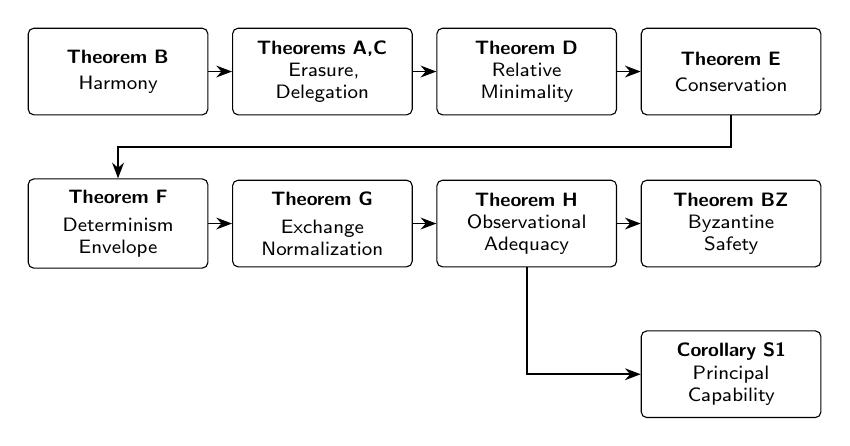
\begin{tikzpicture}[figfont, node distance=3mm]
			\def\depboxw{20mm}
			% Main dependency nodes - row 1
			\node[figsubbox, text width=\depboxw, minimum height=11mm] (B)
			{\vspace{-0.3ex}\textbf{Theorem B}\\[0.8ex]Harmony};
			\node[figsubbox, right=3mm of B, text width=\depboxw, minimum height=11mm] (AC)
			{\textbf{Theorems A,C}\\Erasure,\\Delegation};
			\node[figsubbox, right=3mm of AC, text width=\depboxw, minimum height=11mm] (D)
			{\textbf{Theorem D}\\Relative\\Minimality};
			\node[figsubbox, right=3mm of D, text width=\depboxw, minimum height=11mm] (E)
			{\vspace{-0.3ex}\textbf{Theorem E}\\[0.8ex]Conservation};

			% Main dependency nodes - row 2
			\node[figsubbox, below=8mm of B, text width=\depboxw, minimum height=11mm] (F)
			{\textbf{Theorem F}\\[2pt]Determinism\\Envelope};
			\node[figsubbox, right=3mm of F, text width=\depboxw, minimum height=11mm] (G)
			{\textbf{Theorem G}\\[2pt]Exchange\\Normalization};
			\node[figsubbox, right=3mm of G, text width=\depboxw, minimum height=11mm] (H)
			{\textbf{Theorem H}\\Observational\\Adequacy};
			\node[figsubbox, right=3mm of H, text width=\depboxw, minimum height=11mm] (BZ)
			{\textbf{Theorem BZ}\\Byzantine\\Safety};

			% Branch node row
			\node[figsubbox, below=8mm of BZ, text width=\depboxw, minimum height=11mm] (S1)
			{\textbf{Corollary S1}\\Principal\\Capability};

			% Main dependency arrows
			\draw[figarrowstrong] (B) -- (AC);
			\draw[figarrowstrong] (AC) -- (D);
			\draw[figarrowstrong] (D) -- (E);
			\coordinate (EFmid) at ($(E.south)!0.5!(F.north)$);
			\draw[figarrowstrong] (E.south) -- (E.south |- EFmid) -- (F.north |- EFmid) -- (F.north);
			\draw[figarrowstrong] (F) -- (G);
			\draw[figarrowstrong] (G) -- (H);
			\draw[figarrowstrong] (H) -- (BZ);
			\draw[figarrowstrong] (H.south) -- ++(0,-2mm) |- (S1.west);
		\end{tikzpicture}
	}%
	\caption{Theorem dependency graph}
	\label{fig:p3-dependency-graph}
\end{figure}

\begin{proposition}[Regime Monotonicity]
	If a theorem requires regime $R$, then any stronger regime $R'$ with $R \preceq R'$ preserves theorem validity.
\end{proposition}

\begin{proof}[Proof sketch]
	Assume $R \preceq R'$, so $\mathrm{Prem}(R) \subseteq \mathrm{Prem}(R')$ by definition. Any derivation under $R$ uses only premises from $\mathrm{Prem}(R)$, hence all of its premises are available under $R'$. Therefore theorem validity is monotone along the regime order.
\end{proof}

\subsection{Consequence of the Dependency Graph}

Structural theorems (A--D) are insensitive to quantitative profile constants; quantitative and envelope/byzantine claims are regime-indexed exactly as declared in main text assumption blocks.

\section{Deferred Transport Schemas}
\label{app:transport}

Transport results in Section~\ref{sec:transport} factor into structural and analytic layers.

\subsection{Generic Transport Rule}

\begin{theorem}[Transport by Premise Separation]
	\label{thm:app-p3-transport-separation}
	If structural premises of \ABHStack\ hold and analytic package $A_T$ holds for target claim $T$, then $T$ follows without strengthening structural premises.
\end{theorem}

\begin{proof}[Proof sketch]
	Proof mode: interface composition.
	Map the structural side of \ABHStack\ into the interface required by $A_T$ and
	obtain intermediate judgment $\mathsf{IfaceReady}_T$. Apply the analytic
	theorem under $\mathsf{IfaceReady}_T$ to derive claim $T$ in interface form,
	then transport it back to protocol form through the same map. No additional
	structural premise is introduced.
\end{proof}

\subsection{Interface Discipline}

Transport statements must expose only:
\begin{enumerate}
	\item structural interface obligations (coherence/harmony/envelope/adherence),
	\item analytic assumptions external to this manuscript,
	\item resulting transported consequence.
\end{enumerate}

This prevents hidden strengthening of either side.

\subsection{Representative Schemas}

\begin{enumerate}
	\item Tail-bound transport schema:
	      \begin{equation}
		      \begin{aligned}
			      \text{Struct}_{B..H} \land \text{ConcentrationPkg}(\theta)
			       & \Longrightarrow                     \\
			      \forall t \ge 0,\ \Pr[X - \mathbb{E}X \ge t]
			       & \le \Psi_{\mathrm{tail}}(t;\theta).
		      \end{aligned}
	      \end{equation}
	\item Mixing/convergence transport schema:
	      \begin{equation}
		      \begin{aligned}
			      \text{Struct}_{B..H} \land \text{MixPkg}(\eta)
			       & \Longrightarrow                  \\
			      \forall n \ge 0,\ \|\mu_n - \mu_*\|_{\mathrm{TV}}
			       & \le \Psi_{\mathrm{mix}}(n;\eta).
		      \end{aligned}
	      \end{equation}
	\item Compositional exactness transport schema:
	      \begin{equation}
		      \begin{aligned}
			      \text{Struct}_{B..H} \land \text{NonInterference}
			       & \Longrightarrow \\
			      \EnvelopeExact(C_1) \land \EnvelopeExact(C_2)
			       & \Rightarrow     \\
			      \EnvelopeExact(C_1 \otimes C_2).
		      \end{aligned}
	      \end{equation}
	\item Byzantine adherence transport schema:
	      \begin{equation}
		      \begin{aligned}
			      \text{Struct}_{B..H}
			       & \land \text{ABlockD}      \\
			       & \land \text{WitnessPkg}   \\
			       & \Longrightarrow           \\
			      \mathsf{VMByzAdheres}
			       &                           \\
			       & \land \EqsafeConformance.
		      \end{aligned}
	      \end{equation}
\end{enumerate}

\section{Deferred Consequence Statements}
\label{app:consequences}

\subsection{Reconfiguration and Minimality}

\begin{proposition}
	Under Assumption Block~\ref{assump:p3-reconfiguration}, Harmony (Theorem~\ref{thm:harmony}) and Relative Minimality (Theorem~\ref{thm:minimality}) imply that any admissible safe-reconfiguration invariant implies $\Coherent$ and therefore factors through the same canonical safety core.
\end{proposition}

\begin{proof}[Proof sketch]
	Theorem~\ref{thm:minimality} shows that every admissible invariant factors through $\Coherent$. Theorem~\ref{thm:harmony} then gives commutation of reconfiguration steps over that common core. Chaining these two implications yields the proposition.
\end{proof}

\subsection{Envelope and Determinism Boundary}

\begin{proposition}
	Under Assumption Block~\ref{assump:p3-envelope}, Theorem~\ref{thm:envelope} and Theorem~\ref{thm:normalization} jointly characterize determinism modulo exchange/spatial normalization and identify strict boundary witnesses for inadmissible envelope extensions.
\end{proposition}

\begin{proof}[Proof sketch]
	Apply Theorem~\ref{thm:envelope} to obtain exact envelope characterization via soundness, realizability, and maximality. Apply Theorem~\ref{thm:normalization} to identify the normalized observational equalities that hold inside that exact envelope. Combining both gives the claimed determinism boundary statement.
\end{proof}

\subsection{Runtime Adequacy and Admission}

\begin{proposition}
	Under Assumption Block~\ref{assump:p3-adequacy}, Theorem~\ref{thm:adequacy} plus Corollary~\ref{cor:principal} yields principal-capability admission completeness with explicit rejection diagnostics when premise evidence is missing.
\end{proposition}

\begin{proof}[Proof sketch]
	Theorem~\ref{thm:adequacy} yields adequacy and adherence under Assumption Block~\ref{assump:p3-adequacy}. Corollary~\ref{cor:principal} then refines this with principal-capability inference and admission completeness. Together they imply the proposition.
\end{proof}

\subsection{Byzantine Scope Boundary}

\begin{proposition}
	Under Assumption Block~\ref{assump:p3-byzantine}, Theorem~\ref{thm:byzantine} and Corollary~\ref{cor:byzantine-converse} establish exact safety characterization and converse counterexample packaging, but do not establish Byzantine liveness outside declared timing/fairness assumptions.
\end{proposition}

\begin{proof}[Proof sketch]
	Theorem~\ref{thm:byzantine} and Corollary~\ref{cor:byzantine-converse} provide exact Byzantine safety characterization and converse counterexample packaging under Assumption Block~\ref{assump:p3-byzantine}. Section~\ref{sec:limitations} explicitly restricts scope away from weaker timing and fairness assumptions required for Byzantine liveness. Therefore the claimed boundary follows directly.
\end{proof}

\section{Reproducibility}
\label{app:reproducibility}

Reproduction workflow and expected outputs are documented in
\texttt{ARTIFACT.md}. The one-command supplement check is
\texttt{just artifact-check}. Pinned-commit, DOI, and Lean-statistics rows are
synchronized via
\texttt{bash scripts/paper\_repro\_rows.sh --sync papers/paper1.tex papers/paper2.tex papers/paper3.tex}.
Artifact semantics note. The Lean artifact exposes an explicit trace-level
strong fairness predicate (\texttt{StrongFairEnv}) refining weak fairness, and
the default in-memory runtime transport implements minimal per-edge FIFO
enqueue/dequeue behavior.

\begin{table}[H]
	\centering
	\footnotesize
	\begin{tabularx}{\columnwidth}{@{}L{0.34\columnwidth}L{0.61\columnwidth}@{}}
		\toprule
		\thead{Artifact Field} & \thead{Value}                                                                             \\
		\midrule
		Repository             & \url{https://github.com/hxrts/telltale}                                                   \\
		Pinned commit & \texttt{ccddc8ea843684c4}\allowbreak\texttt{d2d018f673c4861d}\allowbreak\texttt{0664e008} \\
		Archival DOI & \texttt{DOI-UNSET} \\
		Lean source statistics & 1303 files, 206913 LOC, axioms: 0, unresolved proof holes (\texttt{sorry}): 0 \\
		\bottomrule
	\end{tabularx}
	\caption{Artifact identity and verification statistics for this draft snapshot.}
\end{table}

\begin{enumerate}
	\item Run \texttt{just artifact-check}. This runs reproducibility row checks, \texttt{just escape}, \texttt{just verify-protocols}, paper builds, and manifest generation.
	\item Before camera-ready submission, set DOI in \texttt{papers/artifact\_metadata.env} and run \texttt{just paper-repro-check-strict}.
\end{enumerate}

% Full-width index on its own page
\clearpage
\onecolumn

\section{Anchor Index}
\label{app:index}

Table~\ref{tab:p3-index} maps paper claims to their Lean anchors and source files. Anchors marked with --- are infrastructure lemmas used in proofs but not tied to a single claim. Claim entries include assumption-block tags in square brackets.
Assumption-tag legend for claim cells: [A1] = Assumption
Block~\ref{assump:p3-reconfiguration}, [A2] = Assumption
Block~\ref{assump:p3-envelope}, [A3] = Assumption
Block~\ref{assump:p3-adequacy}, [A4] = Assumption
Block~\ref{assump:p3-byzantine}.
Functional categories in the table are: Theorems and Runtime Gates. Reading
guide for long names:
\texttt{exchange\_normalization\_of\_e1\_bridge\_premises} packages the
exchange-normalization bridge used in Theorem~\ref{thm:normalization};
\texttt{consensus\_envelope\_exact\_of\_profile} lifts envelope exactness to
profile-indexed distributed settings; and
\texttt{topology\_change\_preserves\_vmc\_equiv\_via\_effect\_bisim} gives the
topology-change preservation law at the VM observational quotient.
Nickname note. For scanning, read
\texttt{exchange\_normalization\_of\_e1\_bridge\_premises} as
``ENorm-bridge'' and
\texttt{topology\_change\_preserves\_vmc\_equiv\_via\_effect\_bisim} as
``Topo-VMC-preservation.'' Long anchors generally follow
\texttt{object\_claim\_via\_bridge} naming.

\begin{table}[H]
	\centering
	\scriptsize
	\setlength{\aboverulesep}{0pt}
	\setlength{\belowrulesep}{0pt}
	\setlength{\extrarowheight}{2pt}
	\begin{tabularx}{\textwidth}{L{0.29\textwidth}L{0.37\textwidth}L{0.06\textwidth}>{\raggedright\arraybackslash}X}
		\toprule
		\thead{Anchor}                                                                               & \thead{Path (relative to \texttt{lean/})}                                                                                         & \thead{Sec.}          & \thead{Claims}                                                                                \\
		\midrule
		\multicolumn{4}{@{}l}{\textit{Theorems}}                                                                                                                                                                                                                                                                                                                 \\
		\rowcolor{gray!8}
		\texttt{link\_harmony\_\allowbreak through\_link}                                            & \texttt{Protocol/\allowbreak Deployment/\allowbreak}\mbox{\texttt{LinkingTheorems.lean}}                                          & \S\ref{sec:theorem-b} & Thm.~\ref{thm:harmony} [A1]                                                                   \\
		\texttt{link\_preserves\_\allowbreak coherent}                                               & \texttt{Protocol/\allowbreak Deployment/\allowbreak}\mbox{\texttt{LinkingCore.lean}}                                              & \S\ref{sec:theorem-b} & Thm.~\ref{thm:harmony} [A1]                                                                   \\
		\rowcolor{gray!8}
		\texttt{effect\_bisim\_\allowbreak congr\_link}                                              & \texttt{Runtime/\allowbreak Proofs/\allowbreak EffectBisim/\allowbreak}\mbox{\texttt{Congruence.lean}}                            & \S\ref{sec:theorem-b} & ---                                                                                           \\
		\texttt{config\_equiv\_iff\_\allowbreak effect\_bisim\_silent}                               & \texttt{Runtime/\allowbreak Proofs/\allowbreak EffectBisim/\allowbreak}\mbox{\texttt{ConfigEquivBridge.lean}}                     & \S\ref{sec:theorem-b} & ---                                                                                           \\
		\rowcolor{gray!8}
		\texttt{coherent\_erasure\_\allowbreak stable}                                               & \texttt{Protocol/\allowbreak Coherence/\allowbreak}\mbox{\texttt{ErasureCharacterization.lean}}                                   & \S\ref{sec:theorem-a} & Thm.~\ref{thm:erasure} [A1]                                                                   \\
		\texttt{safe\_delegation\_\allowbreak local\_necessity}                                      & \texttt{Protocol/\allowbreak Coherence/\allowbreak}\mbox{\texttt{ErasureCharacterization.lean}}                                   & \S\ref{sec:theorem-c} & ---                                                                                           \\
		\rowcolor{gray!8}
		\texttt{safe\_delegation\_\allowbreak to\_footprint}                                         & \texttt{Protocol/\allowbreak Coherence/\allowbreak}\mbox{\texttt{ErasureCharacterization.lean}}                                   & \S\ref{sec:theorem-c} & ---                                                                                           \\
		\texttt{footprint\_to\_\allowbreak safe\_delegation}                                         & \texttt{Protocol/\allowbreak Coherence/\allowbreak}\mbox{\texttt{ErasureCharacterization.lean}}                                   & \S\ref{sec:theorem-c} & Cor.~\ref{cor:footprint} [A1]                                                                 \\
		\rowcolor{gray!8}
		\texttt{safe\_delegation\_\allowbreak iff\_footprint}                                        & \texttt{Protocol/\allowbreak Coherence/\allowbreak}\mbox{\texttt{ErasureCharacterization.lean}}                                   & \S\ref{sec:theorem-c} & Cor.~\ref{cor:footprint} [A1]                                                                 \\
		\texttt{relative\_minimality}                                                                & \texttt{Protocol/\allowbreak Coherence/\allowbreak}\mbox{\texttt{ErasureCharacterization.lean}}                                   & \S\ref{sec:theorem-d} & Thm.~\ref{thm:minimality} [A1]                                                                \\
		\rowcolor{gray!8}
		\texttt{flagship\_composed\_\allowbreak system\_conservation}                                & \texttt{Protocol/\allowbreak Deployment/\allowbreak}\mbox{\texttt{LinkingTheorems.lean}}                                          & \S\ref{sec:theorem-e} & Thm.~\ref{thm:conservation} [A1]                                                              \\
		\texttt{lyapunov\_conserved\_\allowbreak under\_balanced\_\allowbreak delegation}            & \texttt{Runtime/\allowbreak Proofs/\allowbreak}\mbox{\texttt{Lyapunov.lean}}                                                      & \S\ref{sec:theorem-e} & ---                                                                                           \\
		\rowcolor{gray!8}
		\texttt{consensus\_envelope\_\allowbreak exact\_of\_profile}                                 & \texttt{Runtime/\allowbreak Proofs/\allowbreak Adapters/\allowbreak Distributed/\allowbreak}\mbox{\texttt{EnvelopeTheorems.lean}} & \S\ref{sec:theorem-f} & Thm.~\ref{thm:envelope}, Cors.~\ref{cor:transportability}--\ref{cor:embedding} [A2]           \\
		\texttt{failure\_envelope\_\allowbreak maximality\_of\_profile}                              & \texttt{Runtime/\allowbreak Proofs/\allowbreak Adapters/\allowbreak Distributed/\allowbreak}\mbox{\texttt{EnvelopeTheorems.lean}} & \S\ref{sec:theorem-f} & ---                                                                                           \\
		\rowcolor{gray!8}
		\texttt{exchange\_normalization\_\allowbreak of\_e1\_bridge\_premises}                       & \texttt{Runtime/\allowbreak Adequacy/\allowbreak EnvelopeCore/\allowbreak}\mbox{\texttt{ReconfigurationBridge.lean}}              & \S\ref{sec:theorem-g} & Thm.~\ref{thm:normalization} [A2]                                                             \\
		\texttt{spatial\_subtyping\_\allowbreak monotonicity\_of\_e1\_\allowbreak bridge\_premises}  & \texttt{Runtime/\allowbreak Adequacy/\allowbreak EnvelopeCore/\allowbreak}\mbox{\texttt{ReconfigurationBridge.lean}}              & \S\ref{sec:theorem-g} & Thm.~\ref{thm:normalization} [A2]                                                             \\
		\rowcolor{gray!8}
		\texttt{vm\_adequacy\_of\_\allowbreak trace\_consistency}                                    & \texttt{Runtime/\allowbreak Adequacy/\allowbreak}\mbox{\texttt{Adequacy.lean}}                                                    & \S\ref{sec:theorem-h} & Thm.~\ref{thm:adequacy} [A3]                                                                  \\
		\texttt{protocol\_outcome\_\allowbreak effect\_bisim\_of\_\allowbreak observational\_eq}     & \texttt{Runtime/\allowbreak Proofs/\allowbreak}\mbox{\texttt{HandlerEquivalence.lean}}                                            & \S\ref{sec:theorem-h} & ---                                                                                           \\
		\rowcolor{gray!8}
		\texttt{compile\_refines\_\allowbreak observational\_eq\_\allowbreak of\_effect\_bisim}      & \texttt{Runtime/\allowbreak Adequacy/\allowbreak}\mbox{\texttt{CompileRefinesEffectBisim.lean}}                                   & \S\ref{sec:theorem-h} & ---                                                                                           \\
		\texttt{vm\_view\_effect\_bisim\_\allowbreak of\_vmc\_equiv}                                 & \texttt{Runtime/\allowbreak Proofs/\allowbreak}\mbox{\texttt{ObserverProjectionEffectBisim.lean}}                                 & \S\ref{sec:theorem-h} & ---                                                                                           \\
		\rowcolor{gray!8}
		\texttt{vm\_c\_equiv\_of\_\allowbreak vm\_view\_effect\_bisim}                               & \texttt{Runtime/\allowbreak Proofs/\allowbreak}\mbox{\texttt{ObserverProjectionEffectBisim.lean}}                                 & \S\ref{sec:theorem-h} & ---                                                                                           \\
		\texttt{topology\_change\_\allowbreak preserves\_vmc\_equiv\_\allowbreak via\_effect\_bisim} & \texttt{Runtime/\allowbreak Proofs/\allowbreak}\mbox{\texttt{ObserverProjectionEffectBisim.lean}}                                 & \S\ref{sec:theorem-h} & ---                                                                                           \\
		\rowcolor{gray!8}
		\texttt{byzantine\_safety\_\allowbreak exact\_of\_profile}                                   & \texttt{Runtime/\allowbreak Proofs/\allowbreak Adapters/\allowbreak Distributed/\allowbreak}\mbox{\texttt{EnvelopeTheorems.lean}} & \S\ref{sec:theorem-h} & Thm.~\ref{thm:byzantine}, Cor.~\ref{cor:byzantine-converse} [A4]                              \\
		\midrule
		\multicolumn{4}{@{}l}{\textit{Runtime Gates}}                                                                                                                                                                                                                                                                                                            \\
		\rowcolor{gray!8}
		\texttt{canOperateUnder\allowbreak ByzantineEnvelope}                                        & \texttt{Runtime/\allowbreak Proofs/\allowbreak TheoremPack/\allowbreak}\mbox{\texttt{API.lean}}                                   & \S\ref{sec:theorem-h} & Prop.~\ref{prop:capability}, Cor.~\ref{cor:principal}, Prop.~\ref{prop:byzantine-vm} [A3, A4] \\
		\bottomrule
	\end{tabularx}
	\caption{Anchor index.}
	\label{tab:p3-index}
\end{table}

\end{document}
